\documentclass[paper=a4,fontsize=10.5bp,jafontsize=10.5bp,twocolumn]{jlreq}

% ===== Fonts & Language =====
\usepackage[haranoaji,nfssonly]{luatexja-preset}

% ===== Layout (margins tightened to compensate for larger font) =====
\usepackage[top=10mm,bottom=10mm,left=8mm,right=8mm]{geometry}
\usepackage{fancyhdr}
\usepackage{titlesec}
\usepackage{multicol}
\usepackage{enumitem}
\usepackage{float}

% ===== Graphics & Color =====
\usepackage{graphicx}
\usepackage{xcolor}
\usepackage{tikz}
\usetikzlibrary{calc,positioning,arrows.meta,shapes.geometric,decorations.pathreplacing}
\usepackage[most]{tcolorbox}
\usepackage{wrapfig}

% ===== Tables =====
\usepackage{booktabs}
\usepackage{tabularx}
\usepackage{array}

% ===== Hyperlinks =====
\usepackage{hyperref}
\hypersetup{colorlinks=true,linkcolor=blue!60!black,urlcolor=blue!60!black,citecolor=blue!60!black}

% ===== Color definitions =====
\definecolor{mainblue}{HTML}{1A5276}
\definecolor{accentorange}{HTML}{E67E22}
\definecolor{lightbg}{HTML}{F4F6F7}
\definecolor{successgreen}{HTML}{27AE60}
\definecolor{dangerred}{HTML}{E74C3C}
\definecolor{sectionblue}{HTML}{2C3E50}

% ===== Section formatting =====
\titleformat{\section}
  {\Large\bfseries\sffamily\color{mainblue}}
  {\thesection}{0.6em}{}
  [\vspace{-0.6em}\textcolor{mainblue}{\rule{\linewidth}{1.2pt}}]

\titleformat{\subsection}
  {\large\bfseries\sffamily\color{sectionblue}}
  {\thesubsection}{0.5em}{}

\titleformat{\subsubsection}
  {\normalsize\bfseries\sffamily\color{sectionblue}}
  {\thesubsubsection}{0.4em}{}

\titlespacing*{\section}{0pt}{0.5em}{0.2em}
\titlespacing*{\subsection}{0pt}{0.3em}{0.1em}
\titlespacing*{\subsubsection}{0pt}{0.18em}{0.06em}

% ===== Custom boxes =====
\newtcolorbox{keybox}[1][]{
  colback=mainblue!5,colframe=mainblue,
  fonttitle=\bfseries\sffamily,
  title=#1,boxrule=0.8pt,arc=2pt,
  left=3pt,right=3pt,top=2pt,bottom=2pt
}

\newtcolorbox{highlightbox}{
  colback=accentorange!8,colframe=accentorange,
  boxrule=0.8pt,arc=2pt,
  left=3pt,right=3pt,top=2pt,bottom=2pt
}

\newtcolorbox{graybox}{
  colback=lightbg,colframe=lightbg!60!gray,
  boxrule=0.4pt,arc=2pt,
  left=3pt,right=3pt,top=2pt,bottom=2pt
}

% ===== Header / Footer =====
\pagestyle{fancy}
\fancyhf{}
\renewcommand{\headrulewidth}{0.4pt}
\setlength{\headheight}{14pt}
\fancyhead[L]{\small\sffamily\color{gray}未踏IT人材発掘・育成事業 提案書}
\fancyhead[R]{\small\sffamily\color{gray}無限問題作成AI「モンジェネ」}
\fancyfoot[C]{}

% ===== List spacing =====
\setlist{nosep,leftmargin=1.2em}
\setlist[itemize]{label={\color{mainblue}\textbullet}}

% ===== Paragraph =====
\setlength{\parindent}{1em}
\setlength{\parskip}{0pt}

% ===== Column sep =====
\setlength{\columnsep}{4mm}

% ===== Float spacing =====
\setlength{\textfloatsep}{5pt plus 1pt minus 1pt}
\setlength{\floatsep}{4pt plus 1pt minus 1pt}
\setlength{\intextsep}{4pt plus 1pt minus 1pt}
\setlength{\dbltextfloatsep}{5pt plus 1pt minus 1pt}
\setlength{\dblfloatsep}{4pt plus 1pt minus 1pt}
\setlength{\abovecaptionskip}{3pt}
\setlength{\belowcaptionskip}{1pt}

% ===== Pre-save figure for use in twocolumn header =====
\newsavebox{\mongenecompare}
\savebox{\mongenecompare}{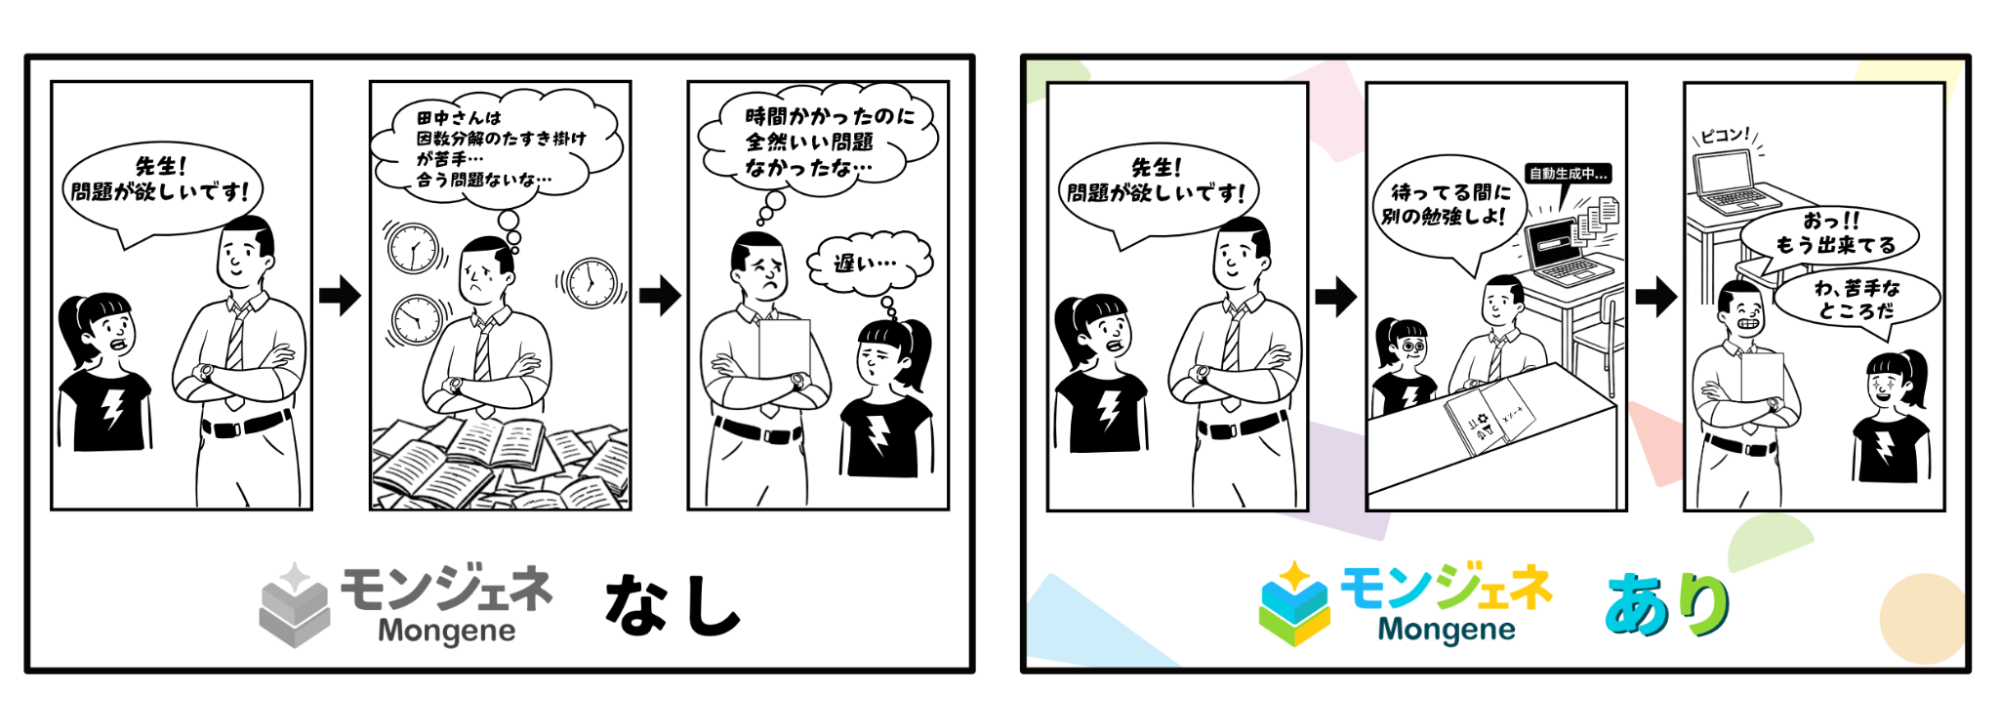
\includegraphics[width=\textwidth]{mongene-compare.png}}

% ============================================================
\begin{document}

% ===== COMPACT HEADER (spans both columns) =====
\twocolumn[
\noindent{\large\sffamily\bfseries\color{mainblue} 生徒ごとに個別最適化された問題生成システムの開発}
\hfill
{\normalsize\sffamily\color{accentorange} 無限問題作成AI「モンジェネ」}\par\vspace{2pt}
{\small\sffamily
\textbf{申請者:} 高橋創真（長岡技術科学大学大学院 修士1年）\quad
\textbf{共同開発者:} 若月耕紀（長岡技科大 院M1）、小武壮太（長岡技科大 院M1）、舛田岳（新潟大 院M1）
}\par\vspace{2pt}
{\small\sffamily 生徒の手書き答案から誤り方と苦手概念を抽出し、講師に「次に教えるべきこと」と「次に出すべき1問」を即時提案する。
AIが講師を置き換えるのではなく、問題探しと採点補助を肩代わりし、講師が生徒に向き合う時間を取り戻す。
未踏期間では、まず\textbf{授業内で本当に使える意思決定支援}を形にする。}\par\vspace{3pt}
{\color{mainblue}\rule{\textwidth}{1.2pt}}
\vspace{0.3em}
\begin{center}
\usebox{\mongenecompare}\par\vspace{1pt}
\refstepcounter{figure}%
{\small\sffamily 図\thefigure：モンジェネの提供価値：問題探しの時間を問題生成に置き換え、講師が生徒と向き合う時間を最大化する}
\label{fig:manga}
\end{center}
\vspace{0.3em}
]


% ============================================================
% ① なにをつくるか
% ============================================================
\section{なにをつくるか}

\subsection{背景}

私が塾講師として最も歯がゆく感じてきたのは、「教えること」が本業であるはずなのに、授業中に\textbf{問題を探す時間}が発生してしまうことである。

私が勤める個別指導塾では、先生1人に生徒2人、1コマは80分間で小学4年生から高校3年生まで指導している。1人の生徒に割ける時間は実質\textbf{40分}だが、解き直し用の問題を紙の問題集から探すだけで\textbf{5〜10分}かかることが珍しくない。つまり、\textbf{指導時間の約25\%}が「紙をめくる時間」に消えている。しかも、やっと見つけた問題が本当にその生徒の苦手に合っているかは、その場では判断しづらい。

\begin{figure}[t]
\centering
\begin{tikzpicture}[font=\scriptsize\sffamily]
  \def\r{1.22}
  \fill[mainblue!15] (0,0) circle (\r);
  \fill[accentorange!85] (0,0) -- (90:\r) arc[start angle=90,end angle=180,radius=\r] -- cycle;
  \draw[mainblue, line width=0.9pt] (0,0) circle (\r);
  \draw[white, line width=1.1pt] (0,0) -- (90:\r);
  \draw[white, line width=1.1pt] (0,0) -- (180:\r);
  \fill[white] (0,0) circle (0.54);
  \node[align=center] at (0,0) {\bfseries 40分\\[-1pt] \tiny 1人あたり};
  \node[align=center, text=accentorange!90!black] at (-1.95,1.05) {\bfseries 問題探し\\10分};
  \node[align=center, text=mainblue!80!black] at (2.08,-0.05) {\bfseries 解説・対話\\30分};
\end{tikzpicture}
\caption{授業時間の内訳イメージ。問題探索だけで約25\%を失っている。}
\label{fig:time_pie}
\end{figure}

この時間を、解説・再説明・励まし・進路相談といった「人にしかできない指導」に戻したい。私は塾講師80名を束ねるリーダーとして同僚を指導するなかで、同じ悩みを持つ講師が多いことを実感している。そこで私たちは、問題を探すのではなく「作ってしまえばよい」と考え、AKATSUKIプロジェクトのひとつであるETSUZAN（新潟県版未踏的人材育成事業）にて、無限問題生成AI「モンジェネ」を開発した。

\subsubsection{ETSUZANでの成果と課題}

モンジェネは、解き直したい問題を入力すると3パターンの類似問題を出力するWebアプリである。

\begin{itemize}
  \item \textbf{パターンA：}数値のみ変更（ケアレスミス克服用）
  \item \textbf{パターンB：}文脈を変更（公式・定理の定着確認用）
  \item \textbf{パターンC：}問われる内容が異なる（解法戦略の強化用）
\end{itemize}

数値計算精度や図形描画精度の課題に対しては、LLMで直接最終文面を生成するのではなく、Pythonコードを生成・外部実行する方式を採用し、「会話なしに一気に問題を作成できる」仕組みを実現した。このモンジェネの使用範囲は高校入学試験対策（中学生用）に限定し、新潟県公立高校入試の空間図形にフォーカスした。

しかし、2026年2月の受験期に使い込むほど、限界も明確になった。難易度を調整できない、出力は固定の3パターンのみ、そして何より---\textbf{生徒一人ひとりの苦手が反映されていない}。私は約20人の生徒を受け持ち、模試・定期テスト・小テストの結果を見ながら個別に対応しているが、20人全員の苦手を正確に把握し続けるのは人間の記憶力だけでは難しい。しかも\textbf{単元が変わるたびに苦手な生徒が入れ替わる}。先月は方程式で苦戦していた生徒が、今月は図形でつまずく。この動的な変化に追従したい、という現場課題が本提案の出発点である。

教育分野では、小中高を対象としたAI活用型の個別学習支援が、学業成績だけでなく自己効力感や学習態度にも一定の改善をもたらすことがレビューで示されている\,[2]。一方で、LLMを教育に用いる近年の研究は、正答を出す能力だけでなく、\textbf{誤り箇所の特定・行動可能なフィードバック・教師による介入設計}が重要だと指摘している\,[3][7][8]。さらに、学生答案の解析、とくに数式誤りや手書き答案の理解は依然として難しく、完全自動化には限界がある\,[9][10]。そこで本提案では、AIが採点を確定するのではなく、\textbf{講師が確認・修正しやすい候補を即時提示する支援システム}として設計する。

本提案の一次目的は、生徒の学力向上をそのままKPIに置くことではない。まずは、講師が\textbf{「次に教える内容」と「次に出す問題」}を短時間で決められる状態をつくることを目標にする。未踏期間では、問題提示までの時間短縮、講師修正率、再出題後の再誤答率を主要指標として検証する。

\subsection{提案システム}

本システムは、塾講師の通常の授業の流れを崩さないことを最優先に設計する。図\ref{fig:cycle}の①〜④の流れで、\textbf{「答案を読む」→「次に教えることを決める」→「次に出す問題を出す」}を授業内で完結させる。

\begin{figure*}[t]
  \centering
  \begin{tikzpicture}[
    font=\small\sffamily,
    stepbox/.style={rectangle, rounded corners=4pt, draw=mainblue, fill=mainblue!5,
      minimum width=3.8cm, minimum height=1.35cm, align=center, line width=0.9pt},
    note/.style={rectangle, rounded corners=4pt, draw=accentorange, fill=accentorange!10,
      minimum width=4.4cm, minimum height=1.1cm, align=center, line width=0.9pt},
    arr/.style={-{Stealth[length=5pt,width=4pt]}, thick, color=gray!70}
  ]
    \node[stepbox] (s1) {① 答案を撮影・アップロード\\[-1pt]\scriptsize 紙の運用はそのまま};
    \node[stepbox, right=0.45cm of s1] (s2) {② 採点候補と苦手仮説\\[-1pt]\scriptsize 正誤・誤り箇所・概念タグ};
    \node[stepbox, right=0.45cm of s2] (s3) {③ 講師への提案\\[-1pt]\scriptsize 次に教える内容と次に出す1問};
    \node[stepbox, right=0.45cm of s3] (s4) {④ 生徒が解き直す\\[-1pt]\scriptsize 結果を次回に反映};
    \node[note, below=0.8cm of s2] (fb) {講師が修正・補足\\[-1pt]\scriptsize このFBが次回の精度向上に効く};

    \draw[arr] (s1) -- (s2);
    \draw[arr] (s2) -- (s3);
    \draw[arr] (s3) -- (s4);
    \draw[arr] (s2) -- (fb);
    \draw[arr] (fb.east) -| ([yshift=-2pt]s3.south);
  \end{tikzpicture}
  \caption{授業内の基本フロー。AIは講師の代わりに教えるのではなく、講師が判断しやすい形で採点候補と対策問題を提示する。}
  \label{fig:cycle}
\end{figure*}

\begin{graybox}
\textbf{未踏期間の主要KPI：}
問題提示までの時間（5〜10分→1分以内）、講師がそのまま採用した提案率、再出題後の同概念での再誤答率。
\end{graybox}


\begin{keybox}[学術的根拠：Bloomの完全習得学習]
教育心理学者 B.\,Bloom\,(1984) は、完全習得学習と1対1個別指導を組み合わせると、平均的な生徒が大きく伸びることを示した\,[1]。近年の小中高向けレビューでも、AIを用いた個別学習支援は学業成績や自己効力感の改善に寄与している\,[2]。本システムは、この個別化を\textbf{講師主導の授業に差し込む}ことを目指す。
\end{keybox}


本提案は\textbf{2つの柱}を掲げる。

\begin{highlightbox}
\begin{enumerate}[leftmargin=2em]
  \item \textbf{個別最適化（パーソナライズ）}：生徒一人ひとりの苦手を高解像度で分析し、その苦手にピンポイントの問題を無限に生成する。
  \item \textbf{完全習得学習（マスタリーラーニング）}：できるようになるまで問題が出てくる。知識グラフで前提概念を管理し、根本原因から段階的に積み上げる。
\end{enumerate}
\end{highlightbox}

\begin{figure*}[t]
  \centering
  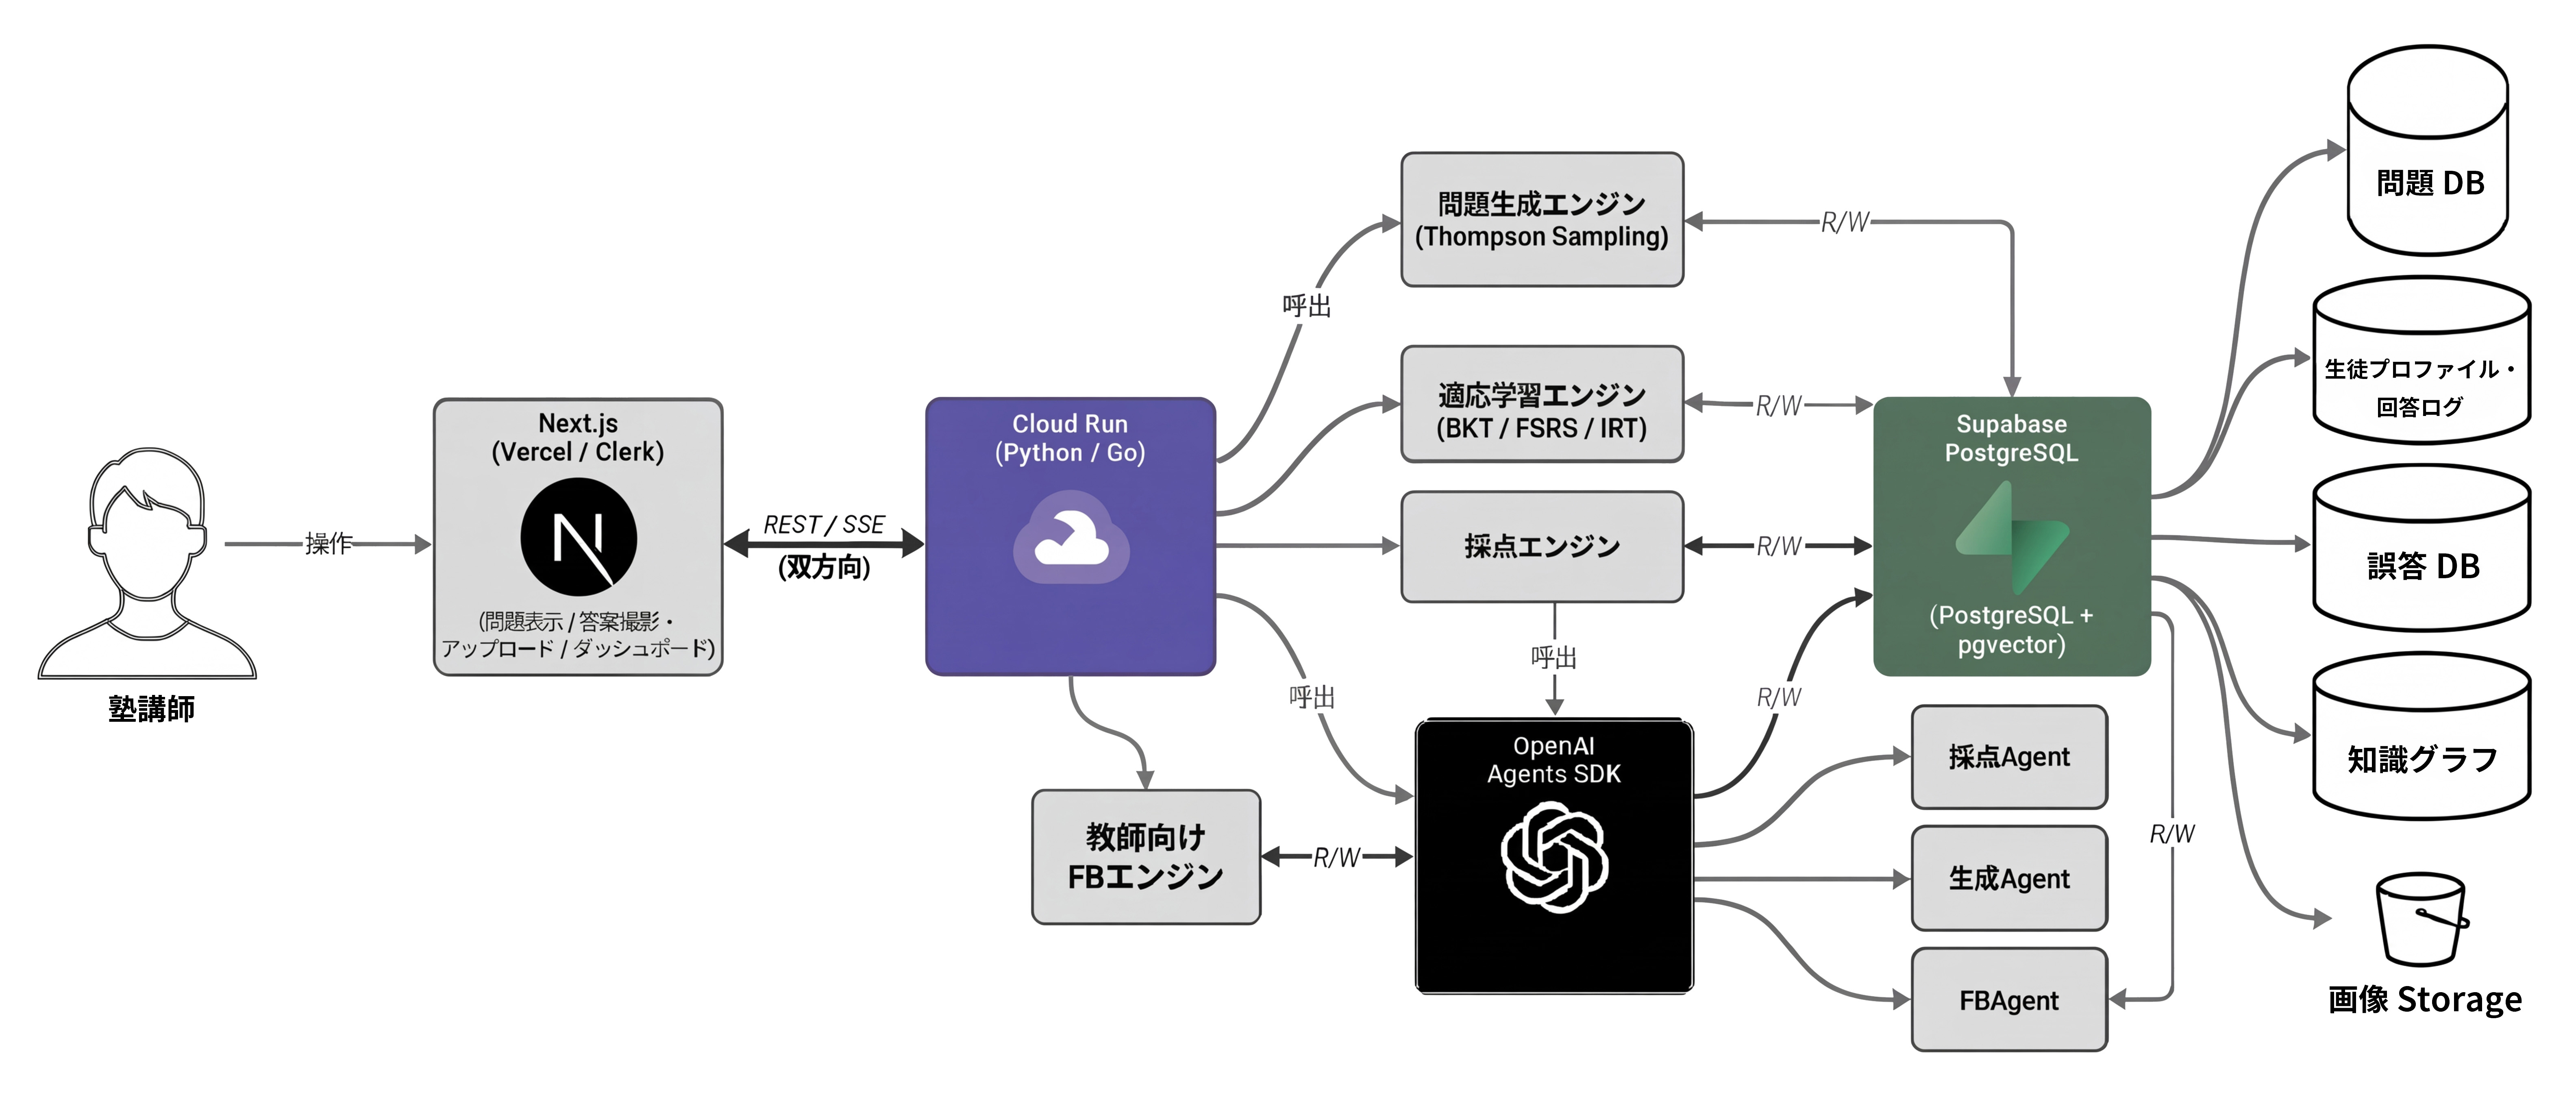
\includegraphics[width=0.80\textwidth]{system-arch-new.jpg}
  \caption{システム全体像：答案解析、苦手推定、問題選定、講師フィードバックをつなぐ。}
  \label{fig:system_overview}
\end{figure*}

以下に、図\ref{fig:system_overview}の処理を抽象から具体へ並べる。

\begin{enumerate}[leftmargin=1.8em]
  \item \textbf{①採点候補の生成}：手書き答案から、正誤候補・誤り箇所・赤入れ案を出す。初期運用では講師が承認して確定する。実装にはマルチモーダルLLMとPython実行環境を用いる。
  \item \textbf{②苦手の推定}：答案を概念タグへ紐づけ、知識グラフとBayesian Knowledge Tracing（BKT）で「どこで止まっているか」を更新する。BKTは少量データでも扱いやすく、講師に説明しやすい確率で表現できる\,[4][5]。
  \item \textbf{③問題の選定・生成}：まずDBから同概念・近い難易度の問題を検索し、不足時のみLLMで新規生成する。生成問題はSymPy等で数式検証し、難易度はIRT較正値と特徴量モデルで推定する。
  \item \textbf{④講師向け提案}：苦手ランキング、次に教えるべき概念、次に出すべき1問を提示する。講師の修正・補足は次回以降の推薦精度向上に返す。
\end{enumerate}

以下、各機能の詳細を述べる。

\subsubsection{【採点・苦手分析エンジン】}

\noindent\textbf{入力：}問題文＋正答、生徒の手書き答案\quad\textbf{出力：}正誤判定、途中式フィードバック、エラー分類

私が所属している塾では、紙とペンで解くこと自体に価値がある。したがって必要なのは、タブレット完結の置き換えではなく、紙の答案を読んだ上で\textbf{講師が判断しやすい採点候補}を返すことである。最新研究でも、学生解答の解析は有望である一方、数式誤りの検出や手書き答案理解には依然として難しさが残る\,[6][9][10]。そのため本システムは完全自動採点ではなく、講師が確認しやすい「正誤候補・誤り箇所・赤入れ案・根拠文」を先に出す設計とする。間違いのタイプは、授業で使いやすい以下の4種類で整理する。

\begin{scriptsize}\noindent
\begin{tabularx}{\linewidth}{>{\bfseries}l X X}
\toprule
エラー分類 & 内容 & 具体例 \\
\midrule
読解・理解エラー & 問題文の読み間違い、求めるものの取り違え & 面積と体積を取り違え \\
変換エラー & 問題を数式に変換する段階でのミス & 「3倍より2大きい」を$3x-2$とする \\
処理エラー & 正しい方針だが計算過程でミス & 移項時の符号ミス、公式の記憶違い \\
書き写しエラー & 途中は正しいが最終解答の転記ミス & 正しい値を途中で出しているのに誤記 \\
\bottomrule
\end{tabularx}
\end{scriptsize}

このエラー分類により、間違いの本質が「知らない」のか、「忘れている」のか、「使い方で止まっている」のかを区別する。この区別が、次の問題選定の精度を決める。

採点結果は蓄積型の\textbf{苦手プロファイル}として記録する。ここでのコールドスタートは、(a) 新規生徒で解答履歴が少ない場合、(b) 新規生成問題で回答履歴がない場合、の2種類である。LLMで問題文・模範解答・答案から概念タグと誤りタイプを初期付与し、その後はBKTで概念ごとの習得確率を更新する\,[4][5]。なお、習得確率85\%は初期閾値であり、未踏期間中に講師修正率と次回正答率を見ながら校正する。性能評価には、教師採点との一致率、エラー分類Macro-F1、講師修正率を用いる。

\subsubsection{【教師向けフィードバック】}

塾講師にとって必要なのは、「授業で何を教えるべきか」の判断材料である。塾講師歴の長さによって、生徒に返せるフィードバックの質は変わる。特に歴の浅い先生にとって、\textbf{どの概念から戻すべきか}を短時間で判断するのは難しい。
本システムは以下を自動生成する。

\begin{itemize}
  \item \textbf{苦手ランキング（優先順位付き）}---志望校の出題傾向を加味して克服すべき苦手を優先順位付け
  \item \textbf{エラーパターンの推移}---直近数週間で「計算ミスは減少」「概念誤解が増加」等のトレンド分析
  \item \textbf{具体的な指導アクション}---根本原因概念、直近の誤りタイプ、志望校・単元進度の3点から、「今回は展開図ではなく三平方の定理から戻す」のような提案を出す
\end{itemize}

さらに、塾講師はフィードバックに対して\textbf{修正・補足を返す}ことができる。この「FBに対するFB」がデータベースに蓄積され、システムの分析精度を継続的に改善する。塾講師の経験知をシステムに還元する双方向ループである。

\subsubsection{【個別最適化問題生成エンジン】}

ETSUZAN期間中に実装した3パターン生成を基盤とし、苦手プロファイルに基づく3つのモードに拡張する。

\begin{scriptsize}\noindent
\begin{tabularx}{\linewidth}{>{\bfseries}l X}
\toprule
モード & 内容 \\
\midrule
苦手克服 & 採点で特定された苦手にピンポイントの問題を生成。知識グラフを遡り根本原因から対処 \\
段階的ステップアップ & 概念ごとに習得度85\%達成まで出題を継続。完全習得学習のAI実装 \\
模試対策 & 志望校の出題傾向・難易度構成を解析し、\textbf{本番と同一構成の模擬テスト一式}を自動生成 \\
\bottomrule
\end{tabularx}
\end{scriptsize}

個別最適化問題の生成では、「元の問題文」「模範解答」「生徒の手書き答案」「採点フィードバック」の4点をLLMに入力し、エラー分類に応じた苦手克服問題を生成する。問題提供は\textbf{検索優先・生成補完}の2段階で行う。まずDBから「同概念・近い難易度・未出題」の候補を検索し、候補が不足する場合のみLLMで新規生成する。生成問題はPythonコード実行による数学的検証を経てから出題し、講師が採用したかどうか、次回正答率が改善したかどうかを記録して比率を更新する。

\subsubsection{【完全習得学習の仕組み】}

苦手をピンポイントで克服できる問題の生成が実現すると、完全習得学習が可能になる。ここでBKTを使う理由は、各概念について「未習得→習得」の確率を逐次更新でき、深層モデルより少量データでも扱いやすく、講師にも説明しやすいためである\,[4]。生徒が確実にできるようになるまで、以下の判定基準でサイクルを繰り返す。

\begin{graybox}
\textbf{習得判定の3条件:}
\begin{enumerate}[leftmargin=2em]
  \item 概念ごとの習得確率（Bayesian Knowledge Tracing）が\textbf{85\%以上}
  \item 直近5問の正答率が\textbf{80\%以上}
  \item \textbf{3問以上}の連続正答
\end{enumerate}
3条件を満たした概念は「習得済み」→次の概念へ。満たさない場合は克服問題を自動提供する。85\%は初期値であり、未踏期間中に実データで校正する。
\end{graybox}

数学の概念には前提関係がある。この前提関係を\textbf{知識グラフ}（有向非巡回グラフ）として管理する。ノードは「平方根の加減」「因数分解の公式適用」のような\textbf{最小概念}、エッジは「これができないと次が解けない」という前提関係である。初期版は学習指導要領・教科書の単元構造・入試問題タグをもとに人手で構築し、各問題を複数ノードに紐づける。

\begin{figure}[t]
\centering
\begin{tikzpicture}[
  node distance=0.35cm and 0.5cm,
  mastered/.style={rectangle, rounded corners=3pt, draw=successgreen, fill=successgreen!10,
    font=\scriptsize\sffamily, minimum height=0.8cm, minimum width=1.5cm, align=center, line width=0.8pt},
  weak/.style={rectangle, rounded corners=3pt, draw=dangerred, fill=dangerred!10,
    font=\scriptsize\sffamily, minimum height=0.8cm, minimum width=1.5cm, align=center, line width=0.8pt},
  progress/.style={rectangle, rounded corners=3pt, draw=accentorange, fill=accentorange!10,
    font=\scriptsize\sffamily, minimum height=0.8cm, minimum width=1.5cm, align=center, line width=0.8pt},
  arr/.style={-{Stealth[length=4pt,width=3pt]}, thick, color=gray!60},
  every node/.append style={inner sep=3pt}
]
  \node[mastered] (sqrt) {平方根\\[-1pt]{\tiny\bfseries\color{successgreen}習得 92\%}};
  \node[weak, right=of sqrt] (factor) {因数分解\\[-1pt]{\tiny\bfseries\color{dangerred}習得 38\%}};
  \node[weak, right=of factor] (quad) {二次方程式\\[-1pt]{\tiny\bfseries\color{dangerred}習得 25\%}};
  \node[weak, right=of quad] (space) {空間図形\\[-1pt]{\tiny\bfseries\color{dangerred}習得 12\%}};
  \node[progress, below=0.6cm of $(factor)!0.5!(quad)$] (pyth) {三平方の定理\\[-1pt]{\tiny\bfseries\color{accentorange}習得 65\%}};
  \draw[arr] (sqrt) -- (factor);
  \draw[arr] (sqrt) -- (pyth);
  \draw[arr] (factor) -- (quad);
  \draw[arr] (pyth) -- (space);
  \draw[arr] (quad) -- (space);
  \node[font=\tiny\sffamily, anchor=north] at ($(factor.south)+(0,-1.2)$) {%
    \textcolor{successgreen}{\rule{5pt}{5pt}}\,習得済\quad
    \textcolor{accentorange}{\rule{5pt}{5pt}}\,学習中\quad
    \textcolor{dangerred}{\rule{5pt}{5pt}}\,苦手};
\end{tikzpicture}
\caption{知識グラフの例：空間図形（習得12\%）でつまずいた生徒の根本原因を因数分解（38\%）まで遡り、そこから段階的に習得させる。}
\label{fig:knowledge_graph}
\end{figure}

生徒がつまずいた場合、知識グラフを遡って根本原因を特定する。空間図形でつまずいている生徒の真の原因が三平方の定理や因数分解の理解不足であれば、まずそこに戻って習得させてから進む。先行の個別学習サービスでも根本原因分析は重要な考え方だが、モンジェネは\textbf{紙の手書き答案}を入力に含め、必要時には\textbf{新規問題を生成できる}点が異なる。

\subsubsection{【データベースの構築】}

蓄積される独自のデータベースによって、このシステムは成長し続ける。

\begin{scriptsize}\noindent
\begin{tabularx}{\linewidth}{>{\bfseries}l X}
\toprule
データ層 & 内容と意義 \\
\midrule
第1層：基盤データ & 統一模試協会の大規模問題データ（正答率付き）、各県入試問題。難易度較正の土台になる \\
第2層：アノテーション & 塾講師が検証した難易度ラベル（正答率5\%刻み21段階）、公式タグ、誤答パターン。LLM構造化出力＋人間検証で構築 \\
第3層：学習効果 & どの問題がどの苦手パターンの生徒に効果があったか。使うほど精度が上がるフライホイール効果 \\
\bottomrule
\end{tabularx}
\end{scriptsize}

DBに蓄積された問題は埋め込みベクトルによるセマンティック検索に対応し、「この生徒の苦手に最も適した問題」を高速に発見する。統一模試データから既存問題のIRT（項目反応理論）困難度を推定し、それを教師信号としてLightGBM回帰を学習する。入力特徴は単元タグ、必要概念数、数式長、図形有無、文章量などであり、これにより\textbf{新規生成問題でも「今の生徒が60〜80\%で解ける帯か」を推定}できる。後発の競合がシステムを模倣しても、このデータ蓄積は即座に再現できない。

\begin{graybox}
\textbf{データの好循環（フライホイール効果）：}
生徒が問題を解く → 回答データが蓄積 → IRT較正の精度向上 → 問題推薦の精度向上 → 学習効果が上がる → ユーザーが増える → さらにデータが蓄積。時間が経つほどシステムの価値が加速度的に高まる。
\end{graybox}

\subsection{未踏期間中の目標}

\begin{enumerate}[leftmargin=2em]
  \item 生徒の手書き答案を採点し、間違えたステップとエラータイプを自動抽出する
  \item 苦手プロファイルに基づく個別最適化問題を生成する
  \item 採点→問題生成のサイクルを塾の現場で実証実験し、問題提示時間・講師修正率・再誤答率を検証する
\end{enumerate}

% ============================================================
\section{どんな出し方を考えているか}

\subsection{公開方法}

Webアプリケーション「モンジェネ」として公開する。塾で用いるタブレット端末やPCでの使用を想定しており、幅広いハードウェアに対応可能なWebアプリが最適である。生徒の手書き答案はスマートフォンやタブレットのカメラで撮影し、アップロードする。紙のワークフローを完全に維持したまま、AIの恩恵を受けられる設計である。

\subsection{ターゲット}

\textbf{未踏期間中}は、提案者代表の高橋が所属する個別指導塾（講師80名・生徒約500名）に限定して検証する。ETSUZAN期間で実証実験を行っており、校長の承認も得ている。ユーザーの声を聞きながらUI/UXを磨き込み、その後の展開に備える。

\textbf{未踏期間後}は、2つのフェーズで展開する。

\begin{enumerate}[leftmargin=2em]
  \item \textbf{Phase 1（地域展開）}：同地域の塾への横展開。新潟県公立高校入試に特化した問題データベースと志望校別の出題傾向分析が差別化要素となる。
  \item \textbf{Phase 2（全国展開）}：各都道府県の入試問題・統一模試データをDBに取り込み、地域ごとの特徴を反映させた全国対応版を提供する。
\end{enumerate}

\subsection{学術的な発表}

本提案では、個別最適化された問題生成と、手書きの解答を採点するという挑戦的な課題を掲げている。本提案はユーザーの負担軽減することが主目的であるため、論文投稿は必要用件ではない。ただユーザーから得られるフィードバックによる検証など、学術的な価値があると判断した際は積極的に学会へ論文を投稿したいと考えている。

未踏に応募する理由は、\textbf{PMの指導のもとで技術を磨き、未踏コミュニティの力を借りて展開を加速したい}からである。自分の塾だけなら未踏なしでも開発を続けられるが、全国の塾に展開するためには、PM・先輩クリエータからのフィードバックと、未踏ブランドによる信頼獲得が不可欠だと考えている。未踏期間後は未踏アドバンストへの進出も視野に入れる。

% ============================================================
\section{斬新さの主張、期待される効果など}

\subsection{既存サービスとの違い}

国内EdTech市場にはatama+やQubenaのような先行サービスが存在する。しかし、これらは\textbf{タブレット完結型}であり、問題供給は主にDB内の既存問題の\textbf{検索・提供}である。モンジェネは知識グラフを用いて生徒の根本原因を特定した上で、その苦手に特化した問題を\textbf{検索し、足りなければ生成する}点が本質的に異なる。

\begin{scriptsize}\noindent
\begin{tabularx}{\linewidth}{>{\bfseries}l X X}
\toprule
比較軸 & atama+\,/\,Qubena & モンジェネ（本提案） \\
\midrule
入力方式 & タブレット操作のみ & \textbf{紙の手書き答案OK} \\
問題供給 & 自社DB内の既存問題を選択 & \textbf{検索＋必要時のみ新規生成} \\
エラー分析 & 正誤＋解答時間＋迷い挙動 & \textbf{途中式を含む誤り候補提示} \\
講師の役割 & 見守り（コーチ） & \textbf{主役（AIのFBを元に解説）} \\
講師の知見還元 & なし（一方通行） & \textbf{FBへのFBでDB改善} \\
導入形態 & タブレット中心 & \textbf{紙＋撮影ベースで導入しやすい} \\
\bottomrule
\end{tabularx}
\end{scriptsize}

\begin{highlightbox}
\textbf{一言で表すなら}：atama+は「タブレットの中の完璧な先生」、モンジェネは「紙の現場に溶け込むAIアシスタント」。既存の紙ベースの指導を活かしたまま、採点と問題生成という最も時間のかかる作業をAIが肩代わりする。塾の指導モデルを置き換えるのではなく、\textbf{講師が生徒と向き合う時間を最大化する}。
\end{highlightbox}

\noindent
加えて、\textbf{開発者自身が5年間の塾講師}であり、「生徒がどこでつまずくか」という肌感覚がシステム設計に直接反映されている点が、技術だけでは到達できない本提案の強みである。

\subsection{期待される効果}

\begin{itemize}
  \item \textbf{一次効果：講師の判断時間の削減}：1コマ40分のうち問題探しに費やす約10分を1分以下に短縮し、解説と対話の時間へ戻す。
  \item \textbf{二次効果：歴の浅い講師の支援}：根本原因概念と次に出す1問が提示されることで、「何を教えるべきか」の判断を平準化できる。
  \item \textbf{中長期効果：学習成果の改善}：AIを用いた個別学習支援は、小中高で学業成績や自己効力感、学習態度の改善が報告されている\,[2]。本システムでも同様の方向性を実証実験で検証する。
\end{itemize}

\subsection{研究・実務から見た妥当性}

教育向けLLM研究では、単に正答を生成することよりも、「どの誤りをどう指摘するか」「行動可能な助言になっているか」を評価する方向へ関心が移っている\,[3][7][8]。一方で、学生答案の解析は依然として難しく、とくに数式誤りや手書き答案では視覚的手がかりが重要である一方、完全自動化には限界がある\,[9][10]。本提案はこの知見に合わせ、\textbf{(1) 対象を中学数学の記述問題に限定し、(2) 講師確認を前提にし、(3) 検索優先・生成補完で安全性を確保する}。

その上で、紙答案の解析、根本原因概念の推定、対策問題の検索／生成を\textbf{授業内の一つのフロー}としてつなぐ点に、本提案の新規性がある。

% ============================================================
\section{具体的な進め方と予算}

\subsection{技術スタックと開発体制}

\begin{scriptsize}\noindent
\begin{tabularx}{\linewidth}{>{\bfseries}l X}
\toprule
領域 & 技術 \\
\midrule
バックエンド & Go (Golang), Python, FastAPI \\
フロントエンド & TypeScript, Next.js \\
AI/ML & OpenAI API, Claude API, Bayesian Knowledge Tracing, IRT, Embedding Search \\
インフラ/DB & AWS or GCP, Supabase (PostgreSQL + pgvector), Vercel \\
認証/決済 & Clerk, Stripe \\
デザイン & Figma \\
\bottomrule
\end{tabularx}
\end{scriptsize}

\subsection{開発チームと役割分担}

\begin{scriptsize}\noindent
\begin{tabularx}{\linewidth}{>{\bfseries}l l X}
\toprule
氏名 & 所属 & 担当 \\
\midrule
高橋創真 & \parbox[t]{3.2cm}{長岡技術科学大学 大学院工学研究科\\工学専攻 情報・経営システム工学分野} & チームマネジメント、ユーザヒアリング、要件定義 \\[4pt]
若月耕紀 & \parbox[t]{3.2cm}{長岡技術科学大学 大学院工学研究科\\工学専攻 情報・経営システム工学分野} & フロントエンド・バックエンド実装全般 \\[4pt]
小武壮太 & \parbox[t]{3.2cm}{長岡技術科学大学 大学院工学研究科\\工学専攻 情報・経営システム工学分野} & UI/UXデザイン、システムデザイン \\[4pt]
舛田　岳 & \parbox[t]{3.2cm}{新潟大学 大学院自然科学研究科\\電気情報工学専攻 情報社会デザイン科学コース 博士前期課程1年} & LLM・ML・インフラ/システム開発全般 \\
\bottomrule
\end{tabularx}
\end{scriptsize}

\subsection{開発スケジュール}

\begin{scriptsize}\noindent
\begin{tabularx}{\linewidth}{>{\bfseries}l X}
\toprule
期間 & マイルストーン \\
\midrule
5月--6月 & 採点エンジンの精度向上。手書き答案のエラー分類精度を検証。統一模試データの取り込みとDB基盤構築 \\
7月--8月 & 苦手プロファイル蓄積機能の実装。知識グラフ（数学の前提概念DAG）構築。塾講師によるアノテーション開始 \\
9月--10月 & 個別最適化問題生成エンジン実装。BKTによる適応的出題。LLM生成問題の数学的検証パイプライン構築 \\
11月--12月 & 教師向けFBダッシュボード実装。完全習得学習フロー（マスタリー判定・矯正問題自動生成）の統合 \\
1月--2月 & 塾での実証実験（講師80名・生徒500名規模）。A/Bテストによる学習効果の定量評価と改善サイクル \\
\bottomrule
\end{tabularx}
\end{scriptsize}

\noindent
各マイルストーンではPM面談でのデモを通じてフィードバックを受け、方針を柔軟に修正する。特に1月--2月の実証実験では、塾講師と生徒双方からのヒアリングを重点的に行い、「現場で本当に使われるか」を最重要KPIとして検証する。

\subsection{計算機環境・開発時間}

\noindent\textbf{計算機環境：}Google Cloud（Cloud Run, Ubuntu）上で開発・デプロイ。メンバーはMacBook Pro等ノートPCを使用。

\noindent\textbf{開発時間：}チームは大学院生4名で構成され、全員が授業単位を取得済みで修士研究のみを抱える状態である。1名あたり週10時間、36週、4名$\times$360時間$=$\textbf{1,440時間}の開発工数を投入する。平日夜間および土日を中心に開発し、1月--2月の実証実験期は塾での検証に時間を重点配分する。

\subsection{予算内訳}

\begin{scriptsize}\noindent
\begin{tabularx}{\linewidth}{>{\bfseries}l r X}
\toprule
費目 & 金額 & 内訳 \\
\midrule
人件費 & 3,024,000円 & 4名 $\times$ 360h $\times$ 2,100円/h \\
クラウド・API利用料 & 200,000円 & LLM API（OpenAI, Claude等）のトークン消費 \\
サーバー・DB維持費 & 100,000円 & 本番/開発環境のインフラ費用 \\
\midrule
\textbf{合計} & \textbf{3,324,000円} & 上限超過分は私費で賄い、\textbf{3,024,000円}を申請 \\
\bottomrule
\end{tabularx}
\end{scriptsize}

\subsection{準備状況}

ETSUZANで開発した「モンジェネ」はデプロイ済みであり、問題生成機能は実稼働している。また、採点システム「ScoGene」のプロトタイプも構築が完了している（\url{https://scogene.vercel.app}）。

\begin{graybox}
\scriptsize\sffamily
\textbf{モンジェネ体験用：}\url{https://mon-gene.wakatsuki.app/login}\quad ID: 77777 / Pass: 20260312\\
\textbf{サンプル問題：}\url{https://drive.google.com/drive/folders/1IaukQ5o0XN11K0-HFi_p95K5nkjOLgd1}\\
\textbf{採点「ScoGene」：}\url{https://scogene.vercel.app}（現状ログインなし）
\end{graybox}

\noindent\textbf{モンジェネの使い方：}ログイン→問題生成ページでサンプル問題の問題と解答をアップロード→類似問題生成→完了後すぐ印刷可能

\noindent\textbf{スコジェネの使い方：}ブラウザで開く→サンプル問題と解答をアップロード→採点開始→完了後、フィードバックが出力

\begin{figure*}[t]
  \centering
  \begin{minipage}[t]{0.32\textwidth}
    \centering
    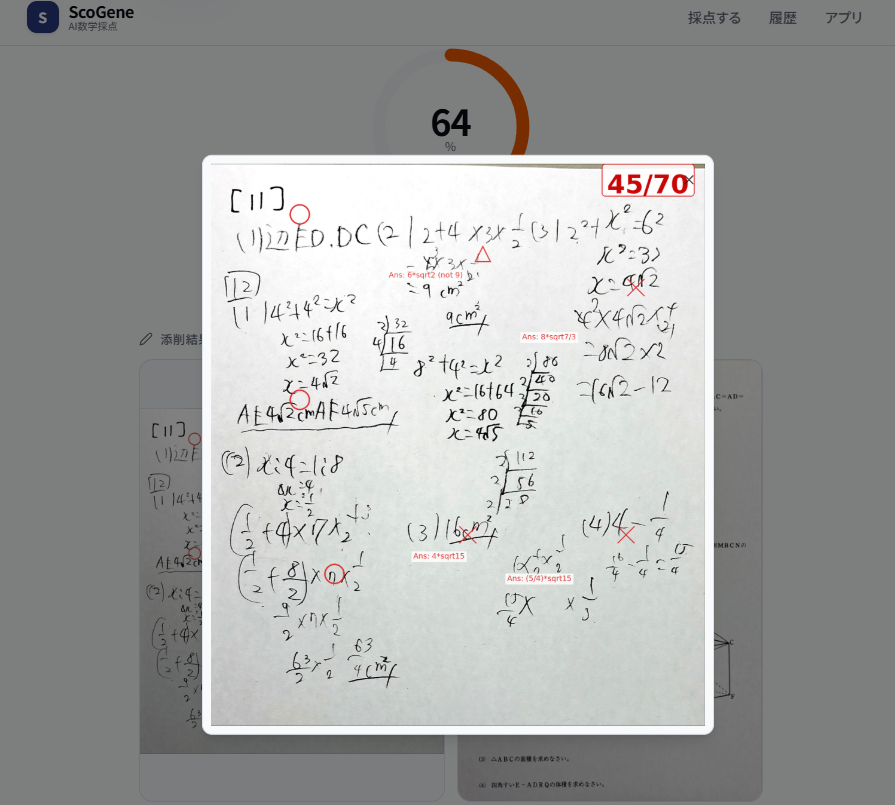
\includegraphics[width=\textwidth]{docs-scogene-overview.png}
    \caption{手書き答案の\\AI採点画面}
    \label{fig:grading_overview}
  \end{minipage}
  \hfill
  \begin{minipage}[t]{0.32\textwidth}
    \centering
    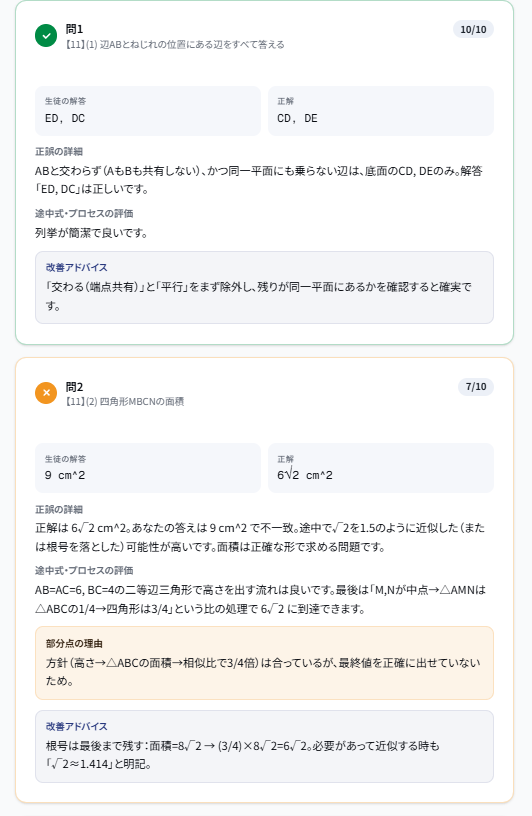
\includegraphics[width=\textwidth]{docs-scogene-detail1.png}
    \caption{採点結果の\\詳細フィードバック}
    \label{fig:grading_detail}
  \end{minipage}
  \hfill
  \begin{minipage}[t]{0.32\textwidth}
    \centering
    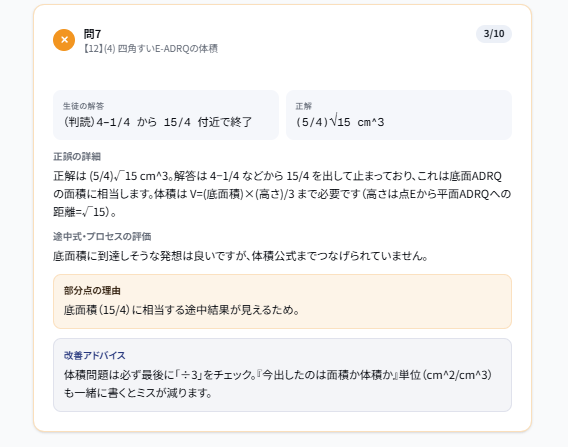
\includegraphics[width=\textwidth]{docs-scogene-detail2.png}
    \caption{途中式評価と\\改善アドバイス}
    \label{fig:grading_feedback}
  \end{minipage}
\end{figure*}

図\ref{fig:grading_overview}--\ref{fig:grading_feedback}に採点プロトタイプの画面を示す。問題文と答案のみを入力し（模範解答を渡していない状態でも）、LLMが正答候補を生成し、生徒の手書き答案から途中式を読み取っている。各問題に対して正誤候補、途中式・プロセスの評価、部分点の理由、改善アドバイスを構造化して出力する。

% ============================================================
\section{提案者（たち）の腕前を証明できるもの}

本チームは、ドメイン知識（塾講師5年）、フルスタック開発力、デザイン力、AI/MLエンジニアリングの4つの専門性がバランスよく揃った構成である。全員が経産省AKATSUKI事業 ETSUZANの採択者であり、開発・発表の実績を持つ。

\begin{graybox}
\scriptsize\sffamily
\textbf{ETSUZAN Makers：}\url{https://meikan.etsuzan.org/}\\
\textbf{発表動画：}モンジェネ \url{https://youtu.be/PCIbYSYGWrI} / SakeScope \url{https://youtu.be/noTHRUNfiwA}\\
\textbf{テレビ放映（舛田 独占取材）：}\url{https://youtu.be/LLsKAEKmDJ4}
\end{graybox}

\begin{figure*}[t]
  \centering
  \begin{minipage}[t]{0.48\textwidth}
    \centering
    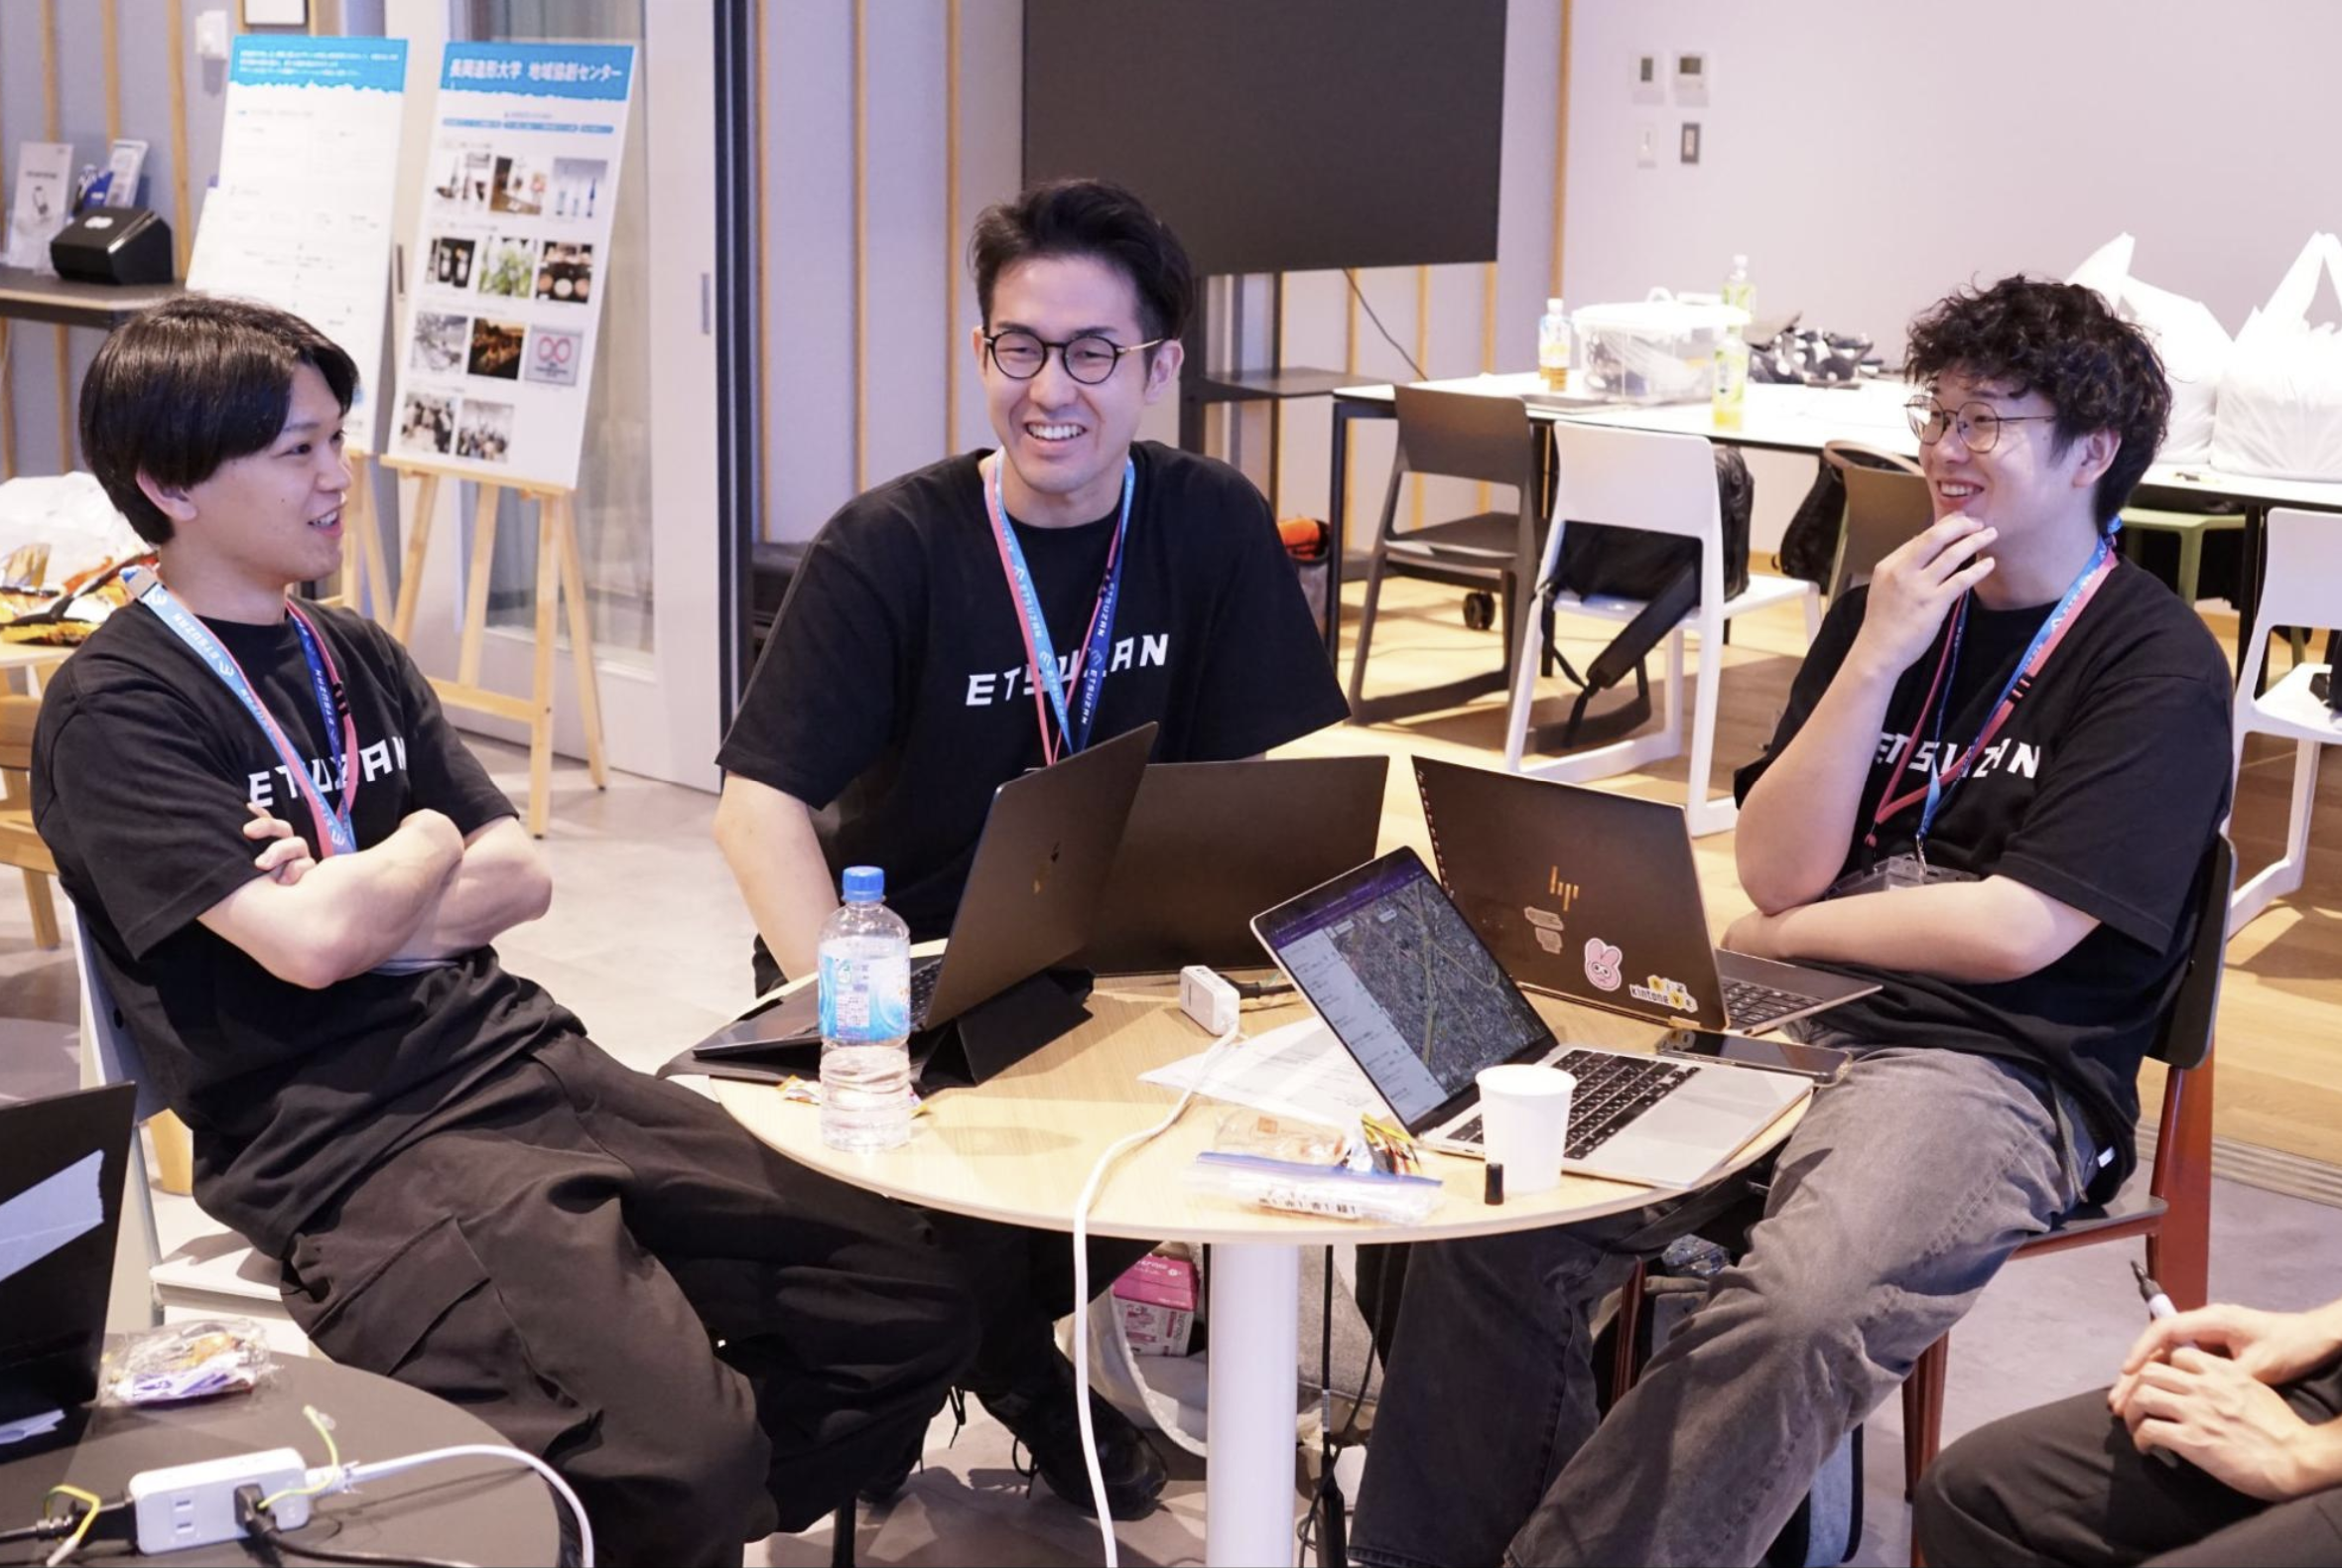
\includegraphics[width=\textwidth]{etsuzan-team.png}
    \caption{ETSUZANでの開発風景}
  \end{minipage}
  \hfill
  \begin{minipage}[t]{0.48\textwidth}
    \centering
    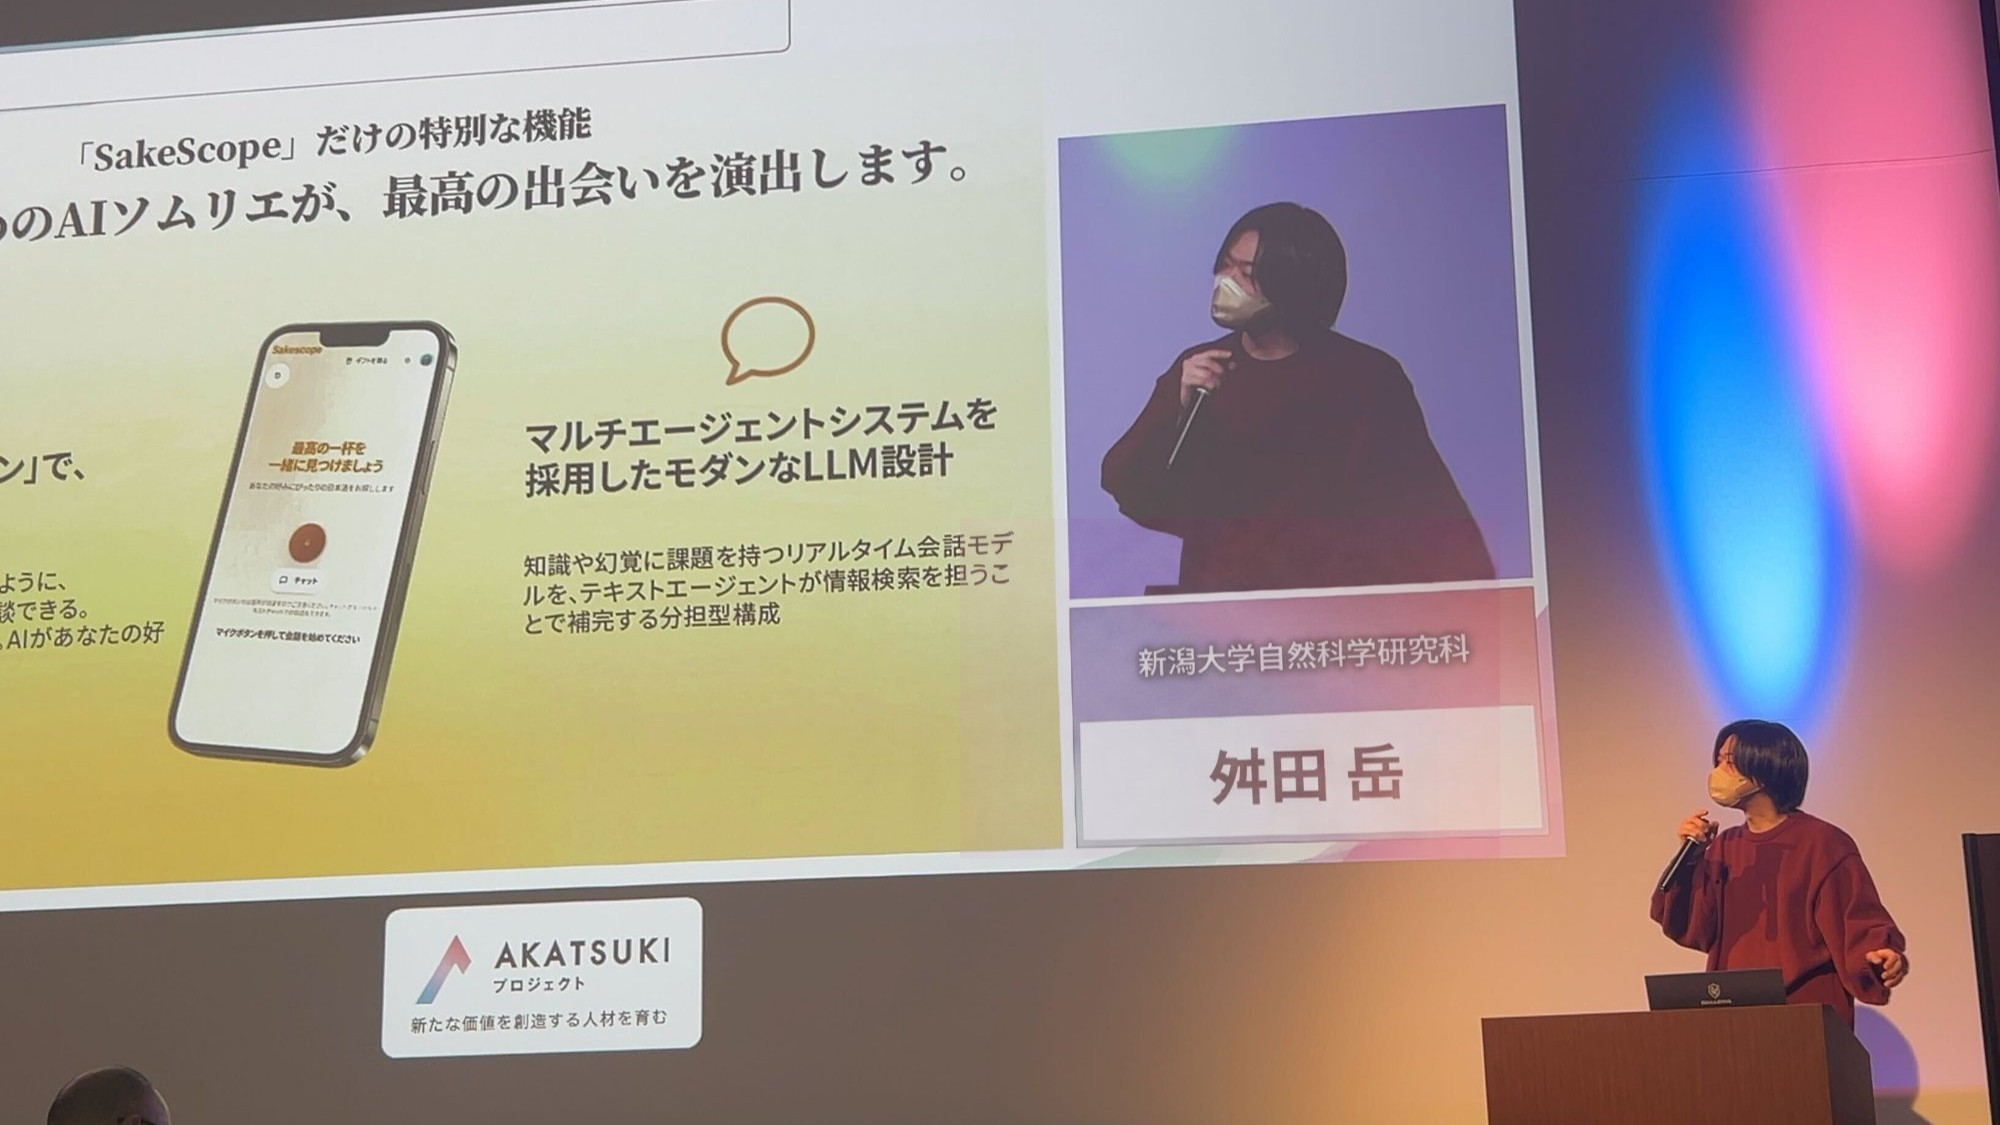
\includegraphics[width=\textwidth]{akatsuki-masuda.jpg}
    \caption{AKATSUKIカンファレンスで\\舛田が代表登壇}
  \end{minipage}
\end{figure*}

\subsection*{高橋 創真}

\noindent\textbf{ETSUZAN採択}\\
\textbf{無限問題生成AI「モンジェネ」チームリーダー}

{\small\sffamily
\noindent
ETSUZAN最終報告会 \url{https://youtu.be/PCIbYSYGWrI}\\
ETSUZAN名鑑 \url{https://meikan.etsuzan.org/}
}

\noindent\textbullet\ \textbf{塾講師アルバイト}：新潟県長岡市の個別指導塾で高専4年次から務めている（今年で5年目）。右も左もわからない新人先生時代から始まり、数々の受験期を乗り越え、現在は塾講師80名を束ねるリーダーとして、生徒の将来の選択肢の広がりを提供している。

\noindent\textbullet\ \textbf{学園祭実行委員長}：長岡技術科学大学学園祭「技大祭」の実行委員会に所属。学部4年次、第43回技大祭実行委員長を務めた。1年間、約200名の組織のトップとして、責任ある立場を全うした。

{\small\sffamily
\noindent
長岡技術科学大学広報誌掲載 \url{https://www.nagaokaut.ac.jp/outline/pr/assets/VOS231web.pdf}
}

\begin{wrapfigure}{r}{0.30\columnwidth}
  \centering
  \vspace{-4pt}
  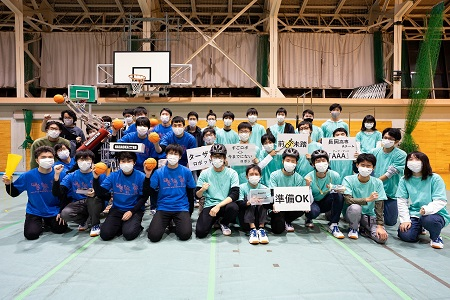
\includegraphics[width=0.28\columnwidth]{docs-robocon.jpg}
  \caption{NHK高専ロボコン2021関東甲信越地区大会}
  \vspace{-8pt}
\end{wrapfigure}

\noindent\textbullet\ \textbf{NHK高専ロボコン}：高専1年から4年まで、NHK高専ロボコンに出場。4年次に、「超絶技巧」がテーマの大会で、前人未踏な「ターザンロボット」を開発。チームリーダー兼部長。地区大会で本田技研工業株式会社特別賞を受賞。1年次は部品加工、2年次はロボット制御プログラムの開発、3年次はチームリーダー。モノづくりの流れを学び、手を動かすことができる実践力を身につけた。

{\small\sffamily
\noindent
高専ロボコン2021関東甲信越地区大会/長岡高専HP \url{https://www.nagaoka-ct.ac.jp/58563/}\\
高専ロボコン2021関東甲信越地区大会アーカイブ \url{https://youtu.be/S-8Iz0e02Xk}
}

\subsection*{若月 耕紀}

\begin{wrapfigure}{r}{0.30\columnwidth}
  \centering
  \vspace{-6pt}
  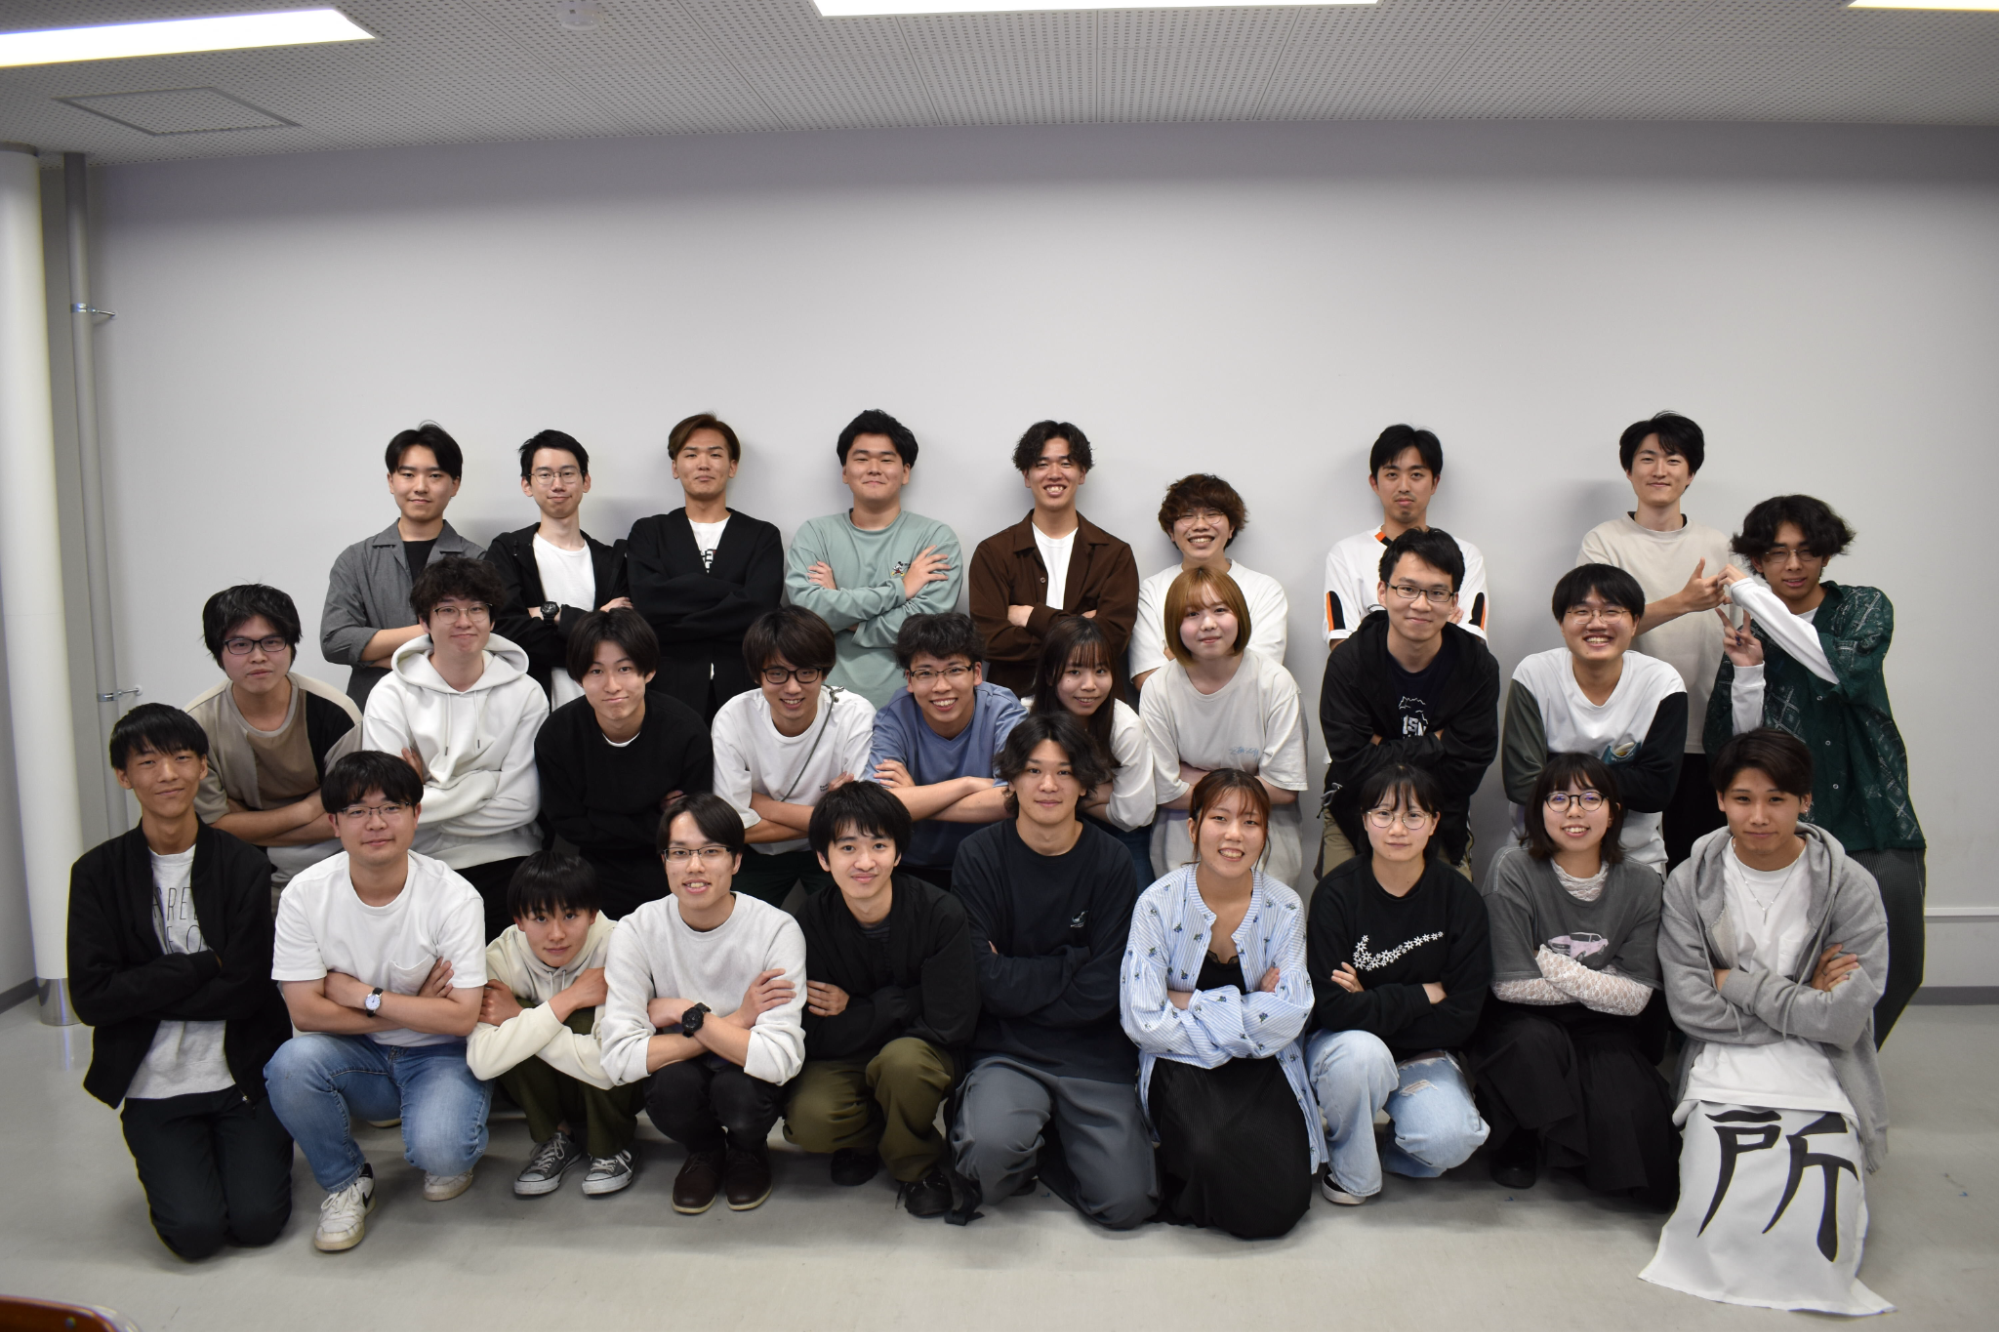
\includegraphics[width=0.28\columnwidth]{docs-nutmeg.png}
  \caption{NUTMEG（技大祭実行委員会 情報局）メンバー}
  \vspace{-8pt}
\end{wrapfigure}

\textbf{【開発実績】}

\noindent\textbullet\ \textbf{NUTMEG}（学園祭実行委員会の開発部門）：シフトの管理・出展団体の管理・組織内の学習コンテンツ管理。Next.jsやRailsなどを用いた、学園祭を支えるアプリケーションの開発。開発団体の代表として、複数プロジェクトをまとめ上げた。

{\small\sffamily
\noindent
NUTMEG公式Blog \url{https://blog.nutmeg.cloud/}
}

\noindent\textbullet\ \textbf{長岡インターンシップサイト}（業務委託）：Web制作会社からの業務委託。要件定義から実装、デプロイまでを1.5ヶ月で完遂。

\noindent\textbullet\ \textbf{モンジェネ}（経産省AKATSUKI事業）：塾講師が抱える「問題不足」という課題に対し、LLMで数学の入試対策問題を無限に生成するアプリケーションを開発。数値計算プログラムや図形描画プログラムを生成させることで、信頼性の高い問題を生成。

\textbf{【研究実績】}
\begin{itemize}
  \item 修士研究テーマ：「GraphVAEを用いたSlackチャットログに基づく組織構造再構成に関する研究」（長岡技術科学大学大学院 情報・経営システム工学分野 機械学習理論研究室）。深層生成モデル（GraphVAE）を用いて、組織内のコミュニケーション構造を可視化・再構成する研究。これにより、組織構造の変革シミュレーションを行う。
\end{itemize}

\subsection*{小武 壮太}

これまで、グラフィックデザインを主軸に、イベントの広報物制作や空間演出のディレクションを行ってきた。現在はその知見をWeb領域へ拡張し、Figmaを用いたUI/UX設計や、生成AIを活用したフロントエンドのプロトタイピングを行っている。以下に主な成果物と関連するリンクを示す。

\begin{itemize}
  \item \textbf{無限問題作成AI『モンジェネ』のUI設計}（ETSUZAN採択）：学習塾講師の業務負荷軽減を目指したWebアプリ。講師の認知負荷と操作コストを下げるため、検索以外のフローをクリック操作のみで完結させるUIを設計した。また、生成AIを活用して自らフロントエンドコードを出力・検証することで、エンジニアへのイメージ共有を円滑にし、開発効率を向上させた。

  \item \textbf{NUTMEG}（長岡技術科学大学 技大祭実行委員会 情報局）での開発：学内団体管理システム「GM2」のフロントエンドを担当。（使用技術: Vue.js, TypeScript）チームメンバーとして、FigmaデザインのUI実装に加え、CSV/PDF出力機能の追加や権限管理の修正などを行った。また、不要コンポーネントの削除やバリデーション修正など、既存コードの保守作業も担当した。

  NUTMEG公式Blog \url{https://blog.nutmeg.cloud/}
\end{itemize}

\subsection*{舛田 岳}

\noindent\textbf{ETSUZAN採択}\\
\textbf{日本酒AIソムリエ「SakeScope」開発者}

{\small\sffamily
\noindent
ETSUZAN最終報告会 \url{https://youtu.be/noTHRUNfiwA}\\
ポートフォリオ \url{https://portfolio.atoriba.jp}
}

\textbf{【開発実績】}
\begin{itemize}
  \item \textbf{社内AIエージェントプラットフォーム}（株式会社b\&qで開発中）：100以上のツール（GWS, GA4, Ahrefs, GSC, Meta Ads等）を統合。Multi-Agent Architecture設計・実装。
  \item \textbf{SEO記事生成SaaS}（株式会社新大陸でテックリード）：LLM、エージェントSDKを活用した記事自動生成システム。月間数千記事の生成実績。
  \item \textbf{SakeScope}（AI日本酒ソムリエ）（経産省AKATSUKI事業）：マルチモーダルLLMによる日本酒推薦システム。地域文化とAIの融合。
\end{itemize}

\textbf{【研究実績】}
\begin{itemize}
  \item 修士研究テーマ：「進化的群知能に基づくLLMエージェント集団の協調最適化」（新潟大学大学院 自然科学研究科 計算知能研究室）。複数のLLMエージェントを進化的アルゴリズムで最適化する研究。
\end{itemize}

% ============================================================
\section{プロジェクト遂行にあたっての特記事項}

現在、高橋、若月、小武は長岡技術科学大学大学院情報・経営システム工学分野修士1年、舛田は新潟大学大学院自然科学研究科修士1年に所属しており、来年度修士2年に進級する。提案者らは共に大学院の授業単位をすべて取り切っており、修士研究を抱えるだけである。研究室の指導教員との関係も良好であり、未踏の応募についても容認されているので、プロジェクト遂行に当たって問題になる可能性は極めて低い。

開発場所は長岡技術科学大学工学研究科 機械学習理論研究室居室、および新潟大学自然科学研究科 計算知能研究室を使用する。高橋は塾に週複数日出勤しており、開発と実証実験のサイクルを高速に回すことが可能である。

\noindent\textbf{チームの経緯：}高橋・若月・小武は長岡技術科学大学の同期であり、学園祭実行委員会（NUTMEG）での開発活動を通じて技術的な信頼関係を構築した。舛田は新潟大学の大学院生で、経産省AKATSUKI事業 ETSUZANにて新潟県の同期採択者として出会い、互いのプロジェクト（モンジェネ・SakeScope）を通じて協力関係を深めた。全員がETSUZAN修了生であり、開発・発表を共にした仲間である。

% ============================================================
\section{IT以外の勉強、特技、生活、趣味}

\subsection*{高橋 創真}

\begin{wrapfigure}{r}{0.42\columnwidth}
  \centering
  \vspace{-6pt}
  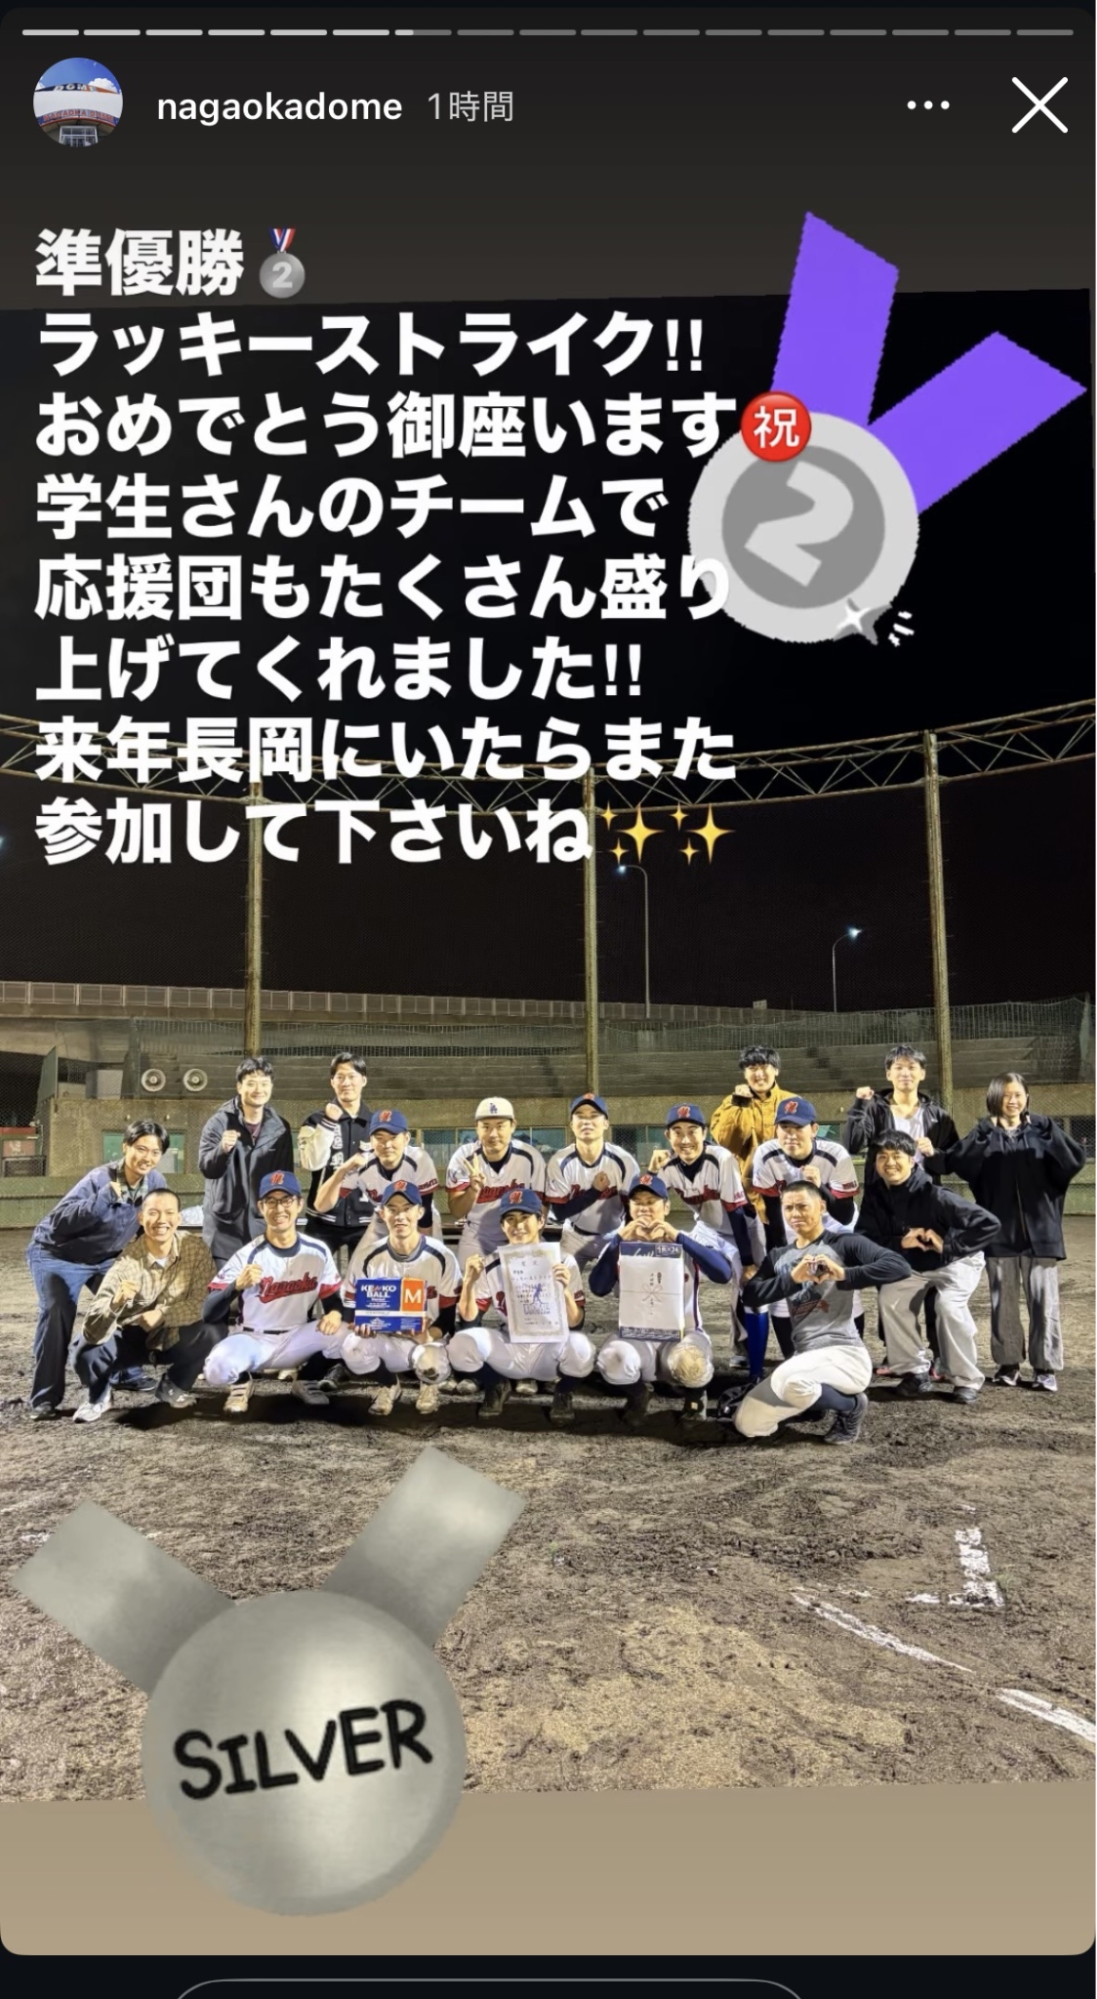
\includegraphics[width=0.40\columnwidth]{docs-hobby-takahashi.png}
  \caption{地域ナイター杯で準優勝}
  \vspace{-6pt}
\end{wrapfigure}

趣味は野球である。小学校3年生から始め、大学院修士1年となった現在も軟式野球部に所属し、精力的に活動している。昨年は、約40チームが出場する地域のナイター杯において、チーム一丸となり準優勝を果たした。プレー面では、体格を活かしたバッティングを持ち味とし、5番レフトとしてチームの勝利に貢献している。もともと私は体力がなく、持久走が大の苦手だったが、鬼監督の厳しい練習を通じて、粘り強い体力と困難に立ち向かう気合を培った。現在は野球に加え、バスケットボールやバレーボールにも挑戦するなど、スポーツ全般を楽しんでいる。今後もスポーツを通じて、心身のタフさを磨き続けたい。

\subsection*{若月 耕紀}

趣味は動物鑑賞である。実家が動物病院を経営しており、生まれた時から動物に囲まれて育った。当時は、犬が9匹、猫が6匹、インコが2羽、うさぎが1羽いた。現在は一人暮らしをしているため、部屋に動物がいない生活を送っている。その反動か、ペットショップや猫カフェなどに行くことが増えた。

\begin{wrapfigure}{r}{0.38\columnwidth}
  \centering
  \vspace{-6pt}
  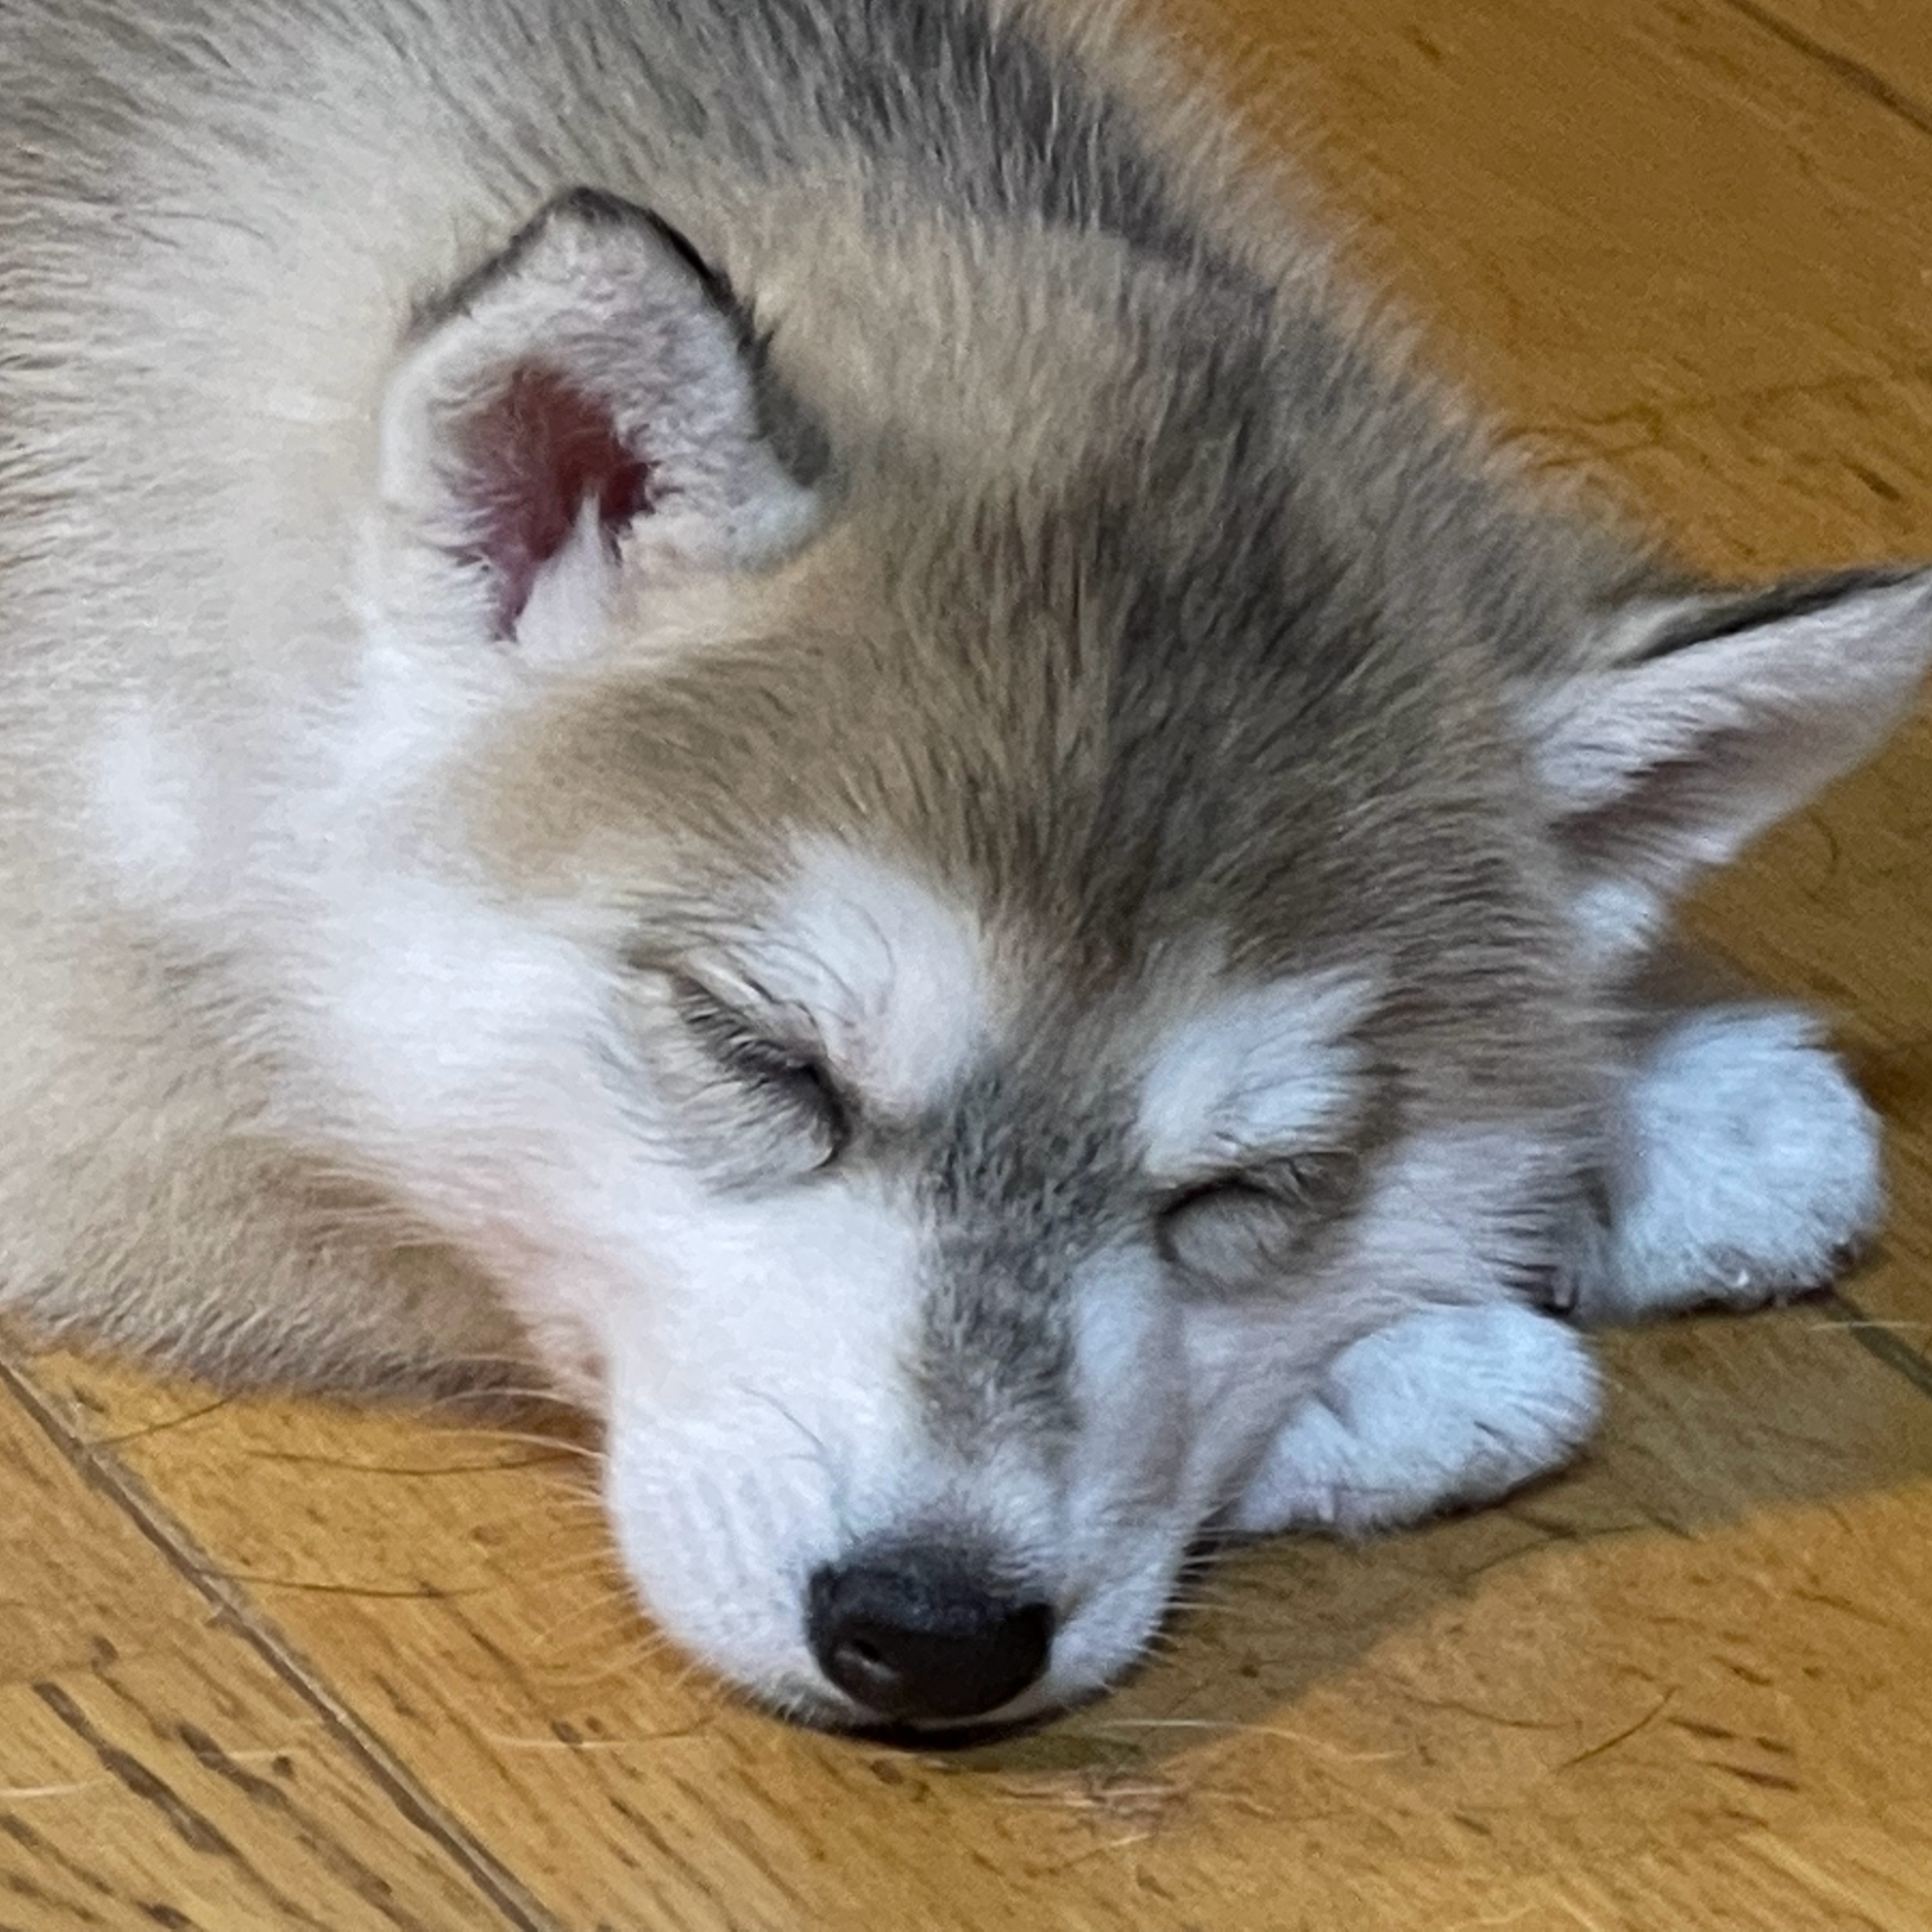
\includegraphics[width=0.36\columnwidth]{docs-hobby-wakatsuki.png}
  \caption{実家の犬}
  \vspace{-6pt}
\end{wrapfigure}

言葉の通じない生き物を相手にすることを、生まれた時から行っていたことが、今のマネジメントスキルにも活きていると考えている。相手が言葉にすることのできない裏側を想像し、引き出す能力につながっていると言える。

\subsection*{小武 壮太}

\begin{wrapfigure}{r}{0.35\columnwidth}
  \centering
  \vspace{-6pt}
  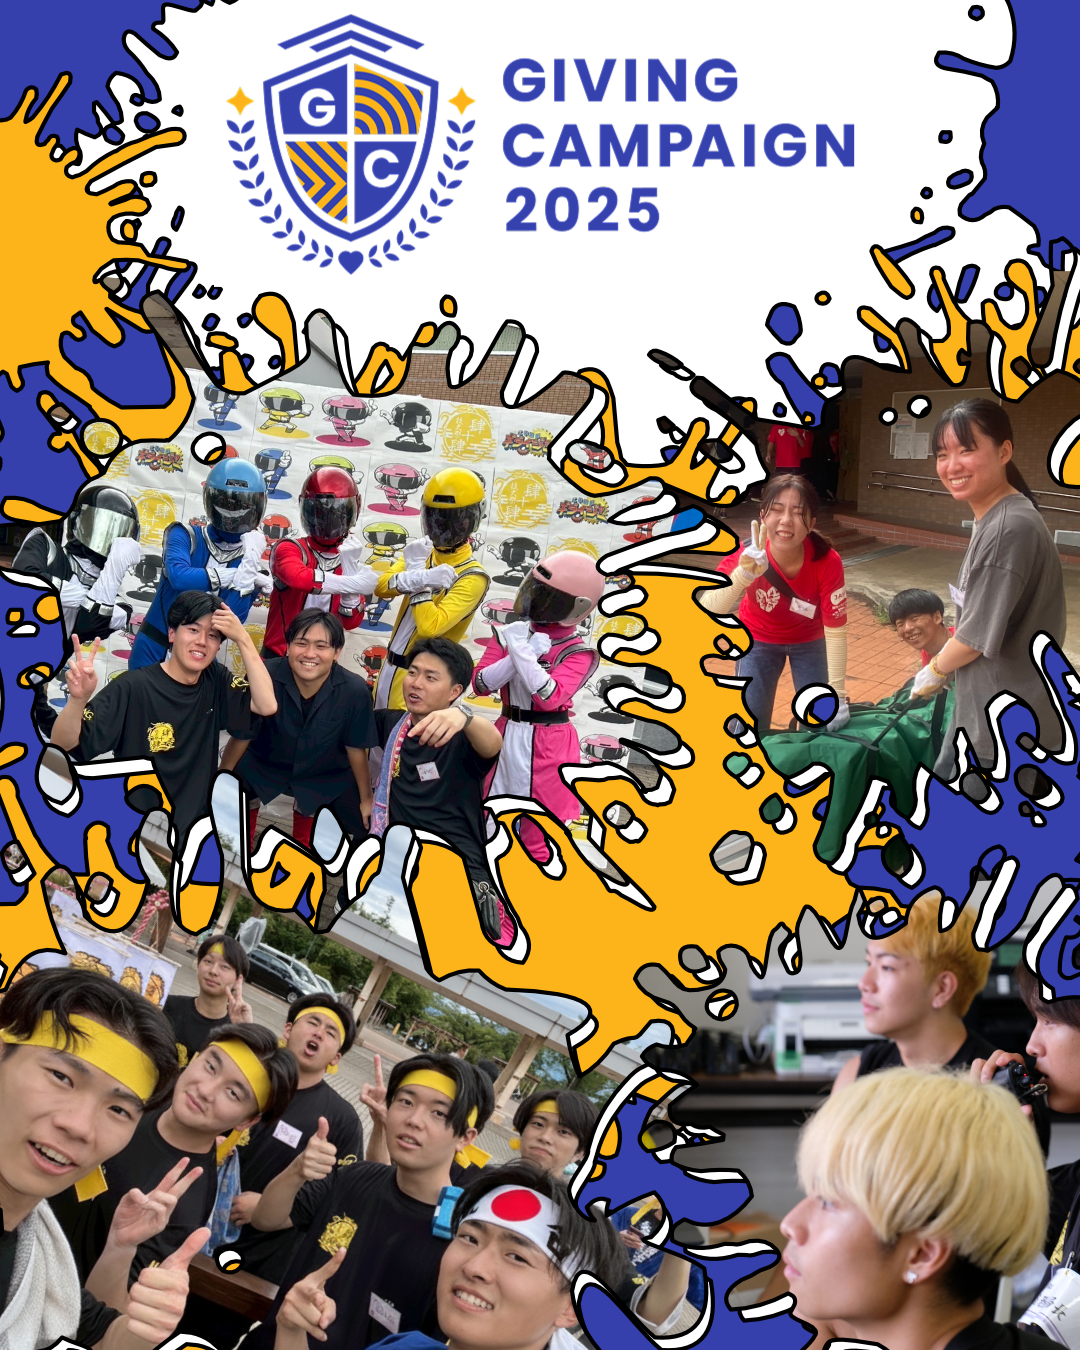
\includegraphics[width=0.33\columnwidth,height=4cm,keepaspectratio]{docs-hobby-kotake.png}
  \caption{技大祭の広報デザイン制作}
  \vspace{-6pt}
\end{wrapfigure}

趣味はデザイン制作である。技大祭実行委員の広報として、Instagramの画像作成や運用といった活動も行っている。依頼者へのヒアリングを通じて企画の意図を深く汲み取り、それを受け手がどう感じるか想像力を巡らせて形にすることにこだわりがある。ぜひ公式アカウント(\url{https://www.instagram.com/nutfes})をご覧いただきたい。この活動で養った「相手の想いを翻訳する力」は、現在のUI/UX設計の根幹を支えている。

\subsection*{舛田 岳}

\begin{wrapfigure}{r}{0.42\columnwidth}
  \centering
  \vspace{-6pt}
  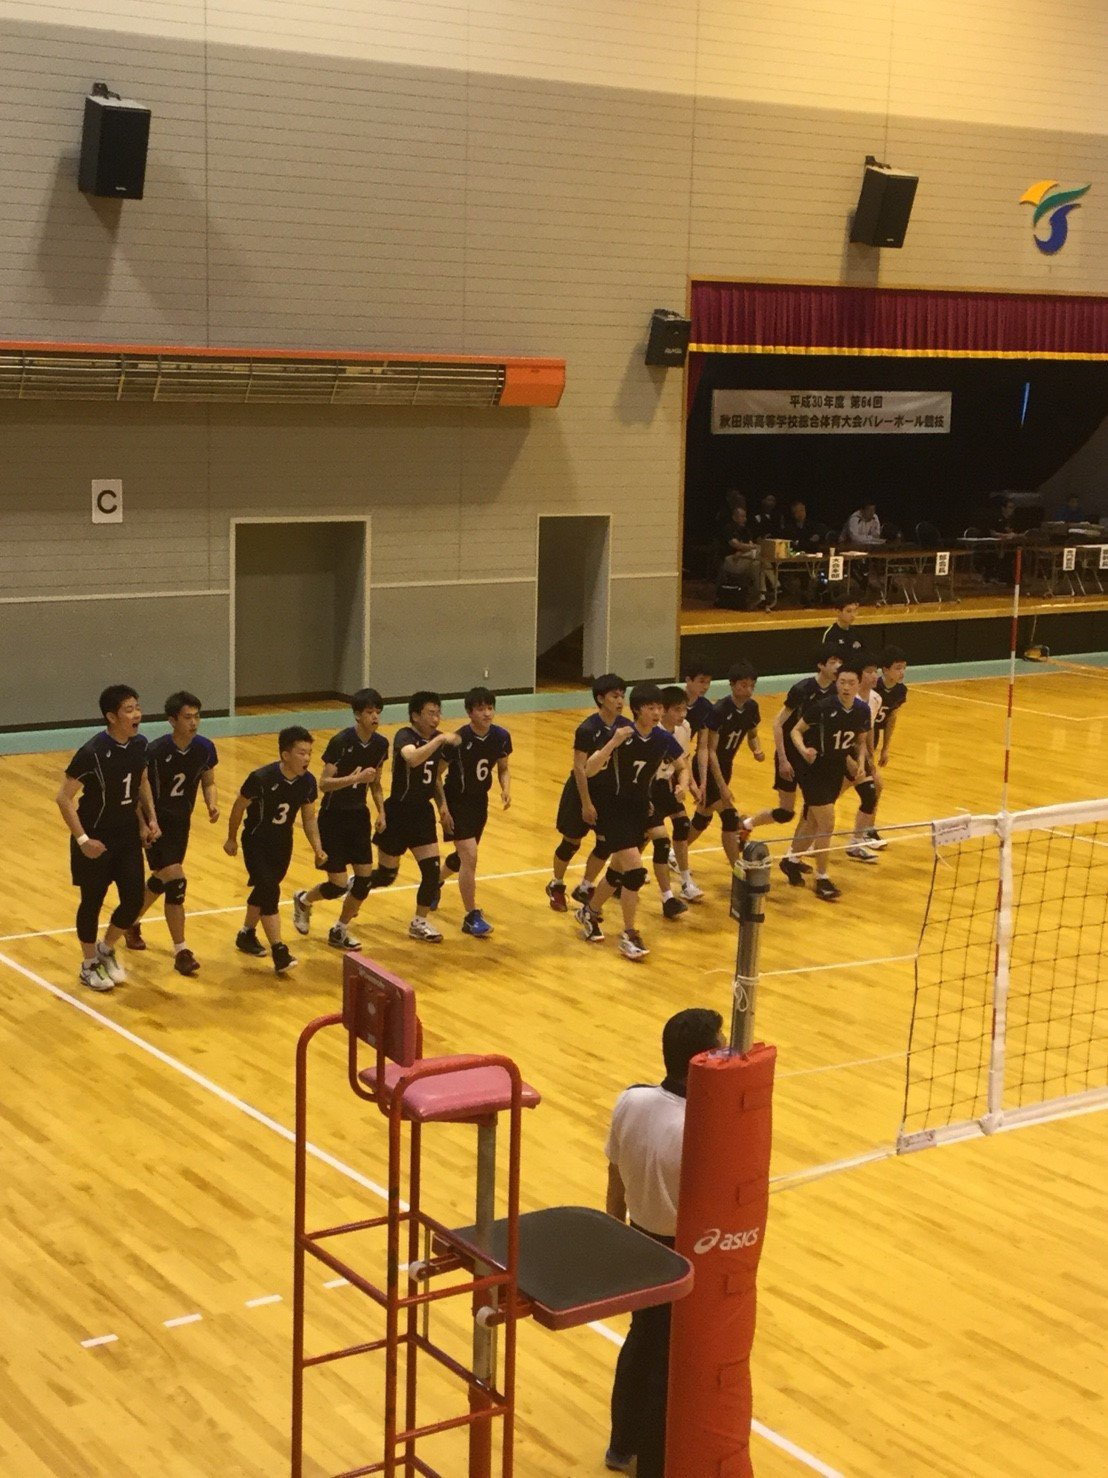
\includegraphics[width=0.40\columnwidth]{docs-hobby-masuda.jpg}
  \caption{高校バレーボール部時代}
  \vspace{-6pt}
\end{wrapfigure}

趣味はバレーボールである。小・中・高と部活動を続け、JOCで秋田県選抜になった経験がある。現在も友人やサークルなどでプレーを続けており、競技としての楽しさはもちろん、チームで連携して結果を出す面白さを大切にしている。

もう一つの趣味は映像制作である。最初は純粋に作ること自体が楽しく、構成・撮影・編集を試しながら学んでいたが、気づけば様々な場面で自然と活用するようになっていた。例えば、バレー部の紹介動画や活動の記録映像、イベントのダイジェストなどを、自ら企画し、撮影し、編集して形にしてきた。「何を、どの順序で、どう見せれば伝わるか」を考えながら制作することは、対象の魅力を引き出し、伝えたい内容を届く形に整える力につながっていると感じている。

% ============================================================
\section{将来のITについて思うこと・期すること}

AIの発展とその応用で様々な作業が効率化しており、省人化無人化になった業務も多いだろう。
人間の学習作業「教育」でもその利用は進んでいるが、教育と人は切り離すことはできない。

誰しも、学生のころ、「この先生の話はちゃんと聞こうかな、、」なんて考えたことがあると思う（あたかも私が先生のことを選んでいるかのように聞こえてしまうが）。この現象は、先生との関係性によって生まれるものである。

教育×ITの取り組みは様々ある。例えば、英語学習を効率的に行えるアプリや常時質問可能なAIチャットがある。いつでもどこでも、時間的空間的な制約無く質問できるなら、もはや先生なんていらないのでは？と考えてしまう。

しかし、生徒の「モチベーション管理」はIT/AIが踏み込めない領域と考える。モチベートの他にも、感情、非合理的な判断、人間関係というのは機械的なものでは構築・理解はできない。AIは生徒と対話することはできても、真にコミュニケーションを取っているとは言えない。さらには、憧れ・夢を抱かせることもできないと考える。

\begin{highlightbox}
\textbf{「憧れや夢は、人と人との関わりのなかで創発する。」}

私はそう考える。

人工知能的な1対1対応（Aと聞いたらBと返ってくる）のAIとの対話は閉じた世界であり、私が言う憧れ/夢は外部から『やってくる』ことはないだろう。
人と人との無限の可能性に満ちた宇宙でこそ、真の教育は生まれる。
教育ITは、\textbf{Human-in-the-Loop}のシステムでなくてはならない。
\end{highlightbox}

モンジェネは、AIが講師を\textbf{置き換える}のではなく、講師が生徒と向き合う時間を\textbf{最大化する}ためのツールである。採点や問題探しという機械的な作業をAIに任せ、解説・動機づけ・進路相談といった「人にしかできない教育」に講師が集中できる世界を、私たちは実現したい。

% ============================================================
\vspace{1em}
\begin{small}
\noindent\textbf{参考文献}
\begin{enumerate}[leftmargin=2em,label={[\arabic*]}]
  \item Bloom, B.\,S. (1984). The 2 Sigma Problem. \textit{Educational Researcher}, 13(6), 4--16.
  \item L\'{e}tourneau, A.\,et~al. (2025). A Systematic Review of AI-Driven ITS in K-12 Education. \textit{npj Science of Learning}, 10, 29.
  \item Pal Chowdhury, S.\,et~al. (2025). Large Language Models for Education: Understanding the Needs of Stakeholders, Current Capabilities and the Path Forward. \textit{Proceedings of the 20th Workshop on Innovative Use of NLP for Building Educational Applications}.
  \item Corbett, A.\,T. \& Anderson, J.\,R. (1994). Knowledge Tracing. \textit{User Modeling and User-Adapted Interaction}, 4, 253--278.
  \item Cho, Y.\,et~al. (2024). A Systematic Review of Knowledge Tracing and Large Language Models in Education. \textit{arXiv:2412.09248}.
  \item Daheim, N.\,et~al. (2024). Stepwise Verification and Remediation of Student Solutions Using Large Language Models. \textit{Proceedings of EMNLP 2024}.
  \item Kochmar, E.\,et~al. (2025). BEA 2025 Shared Task on Pedagogical Ability Assessment of AI Tutors. \textit{Proceedings of the 20th Workshop on Innovative Use of NLP for Building Educational Applications}.
  \item Macina, J.\,et~al. (2025). MathTutorBench: A Benchmark for Measuring Open-ended Pedagogical Capabilities of LLM Tutors. \textit{Proceedings of the 20th Workshop on Innovative Use of NLP for Building Educational Applications}.
  \item Srivatsa, V.\,et~al. (2025). LLMs Cannot Spot Math Errors, but Mathematical Reasoning Can. \textit{arXiv:2506.12173}.
  \item Henkel, O.\,et~al. (2025). Seeing the Big Picture: Visual Reasoning Helps LLMs Analyze Student Work. \textit{arXiv:2510.11124}.
\end{enumerate}
\end{small}

\end{document}
